
\documentclass[aspectratio=169]{beamer}
%\documentclass[compress,aspectratio=169]{beamer}
%%%%%%%%%%%%%%%%%%%%%%%%%%%%%%% Packages %%%%%%%%%%%%%%%%%%%%%%%%%%%%%%%%
\usepackage[utf8]{inputenc}
\usepackage[T1]{fontenc}
\usepackage{graphicx}
\usepackage{ol2a} %ol2a.sty file
\usepackage{multicol}
\usepackage{subfigure}
\usepackage{lmodern}
\usepackage{amsmath}
\usepackage{amssymb}
\usepackage{textcomp}
\usepackage{gensymb}
\usepackage[absolute,overlay]{textpos}
\usepackage{graphicx}
\usepackage{hyperref}
\usepackage[english]{babel}
\usepackage{graphicx,url}
\usepackage{subfigure}
\usepackage{latexsym,amsmath,xcolor,multicol,booktabs,calligra}
\usepackage{graphicx,pstricks,listings,stackengine}
\setbeamertemplate{itemize subitem}{$\rightarrow$}
\usepackage{lipsum}
\usepackage[subnum]{cases}
\usepackage{textpos}
\usepackage{fancybox,calc}
\usepackage{palatino,mathpazo}
\usepackage{amsfonts}
\usepackage{sidecap}
\usepackage{booktabs}
\usepackage{changepage}
%%%%%%%%%%%%%%%%%%%%%%%%%%%%%%% Defs %%%%%%%%%%%%%%%%%%%%%%%%%%%%%%%%
\def\cmd#1{\texttt{\color{orange}\footnotesize $\backslash$#1}}
\def\env#1{\texttt{\color{blue}\footnotesize #1}}
\definecolor{deepblue}{rgb}{0,0,0.5}
\definecolor{deepred}{rgb}{0.6,0,0}
\definecolor{deepgreen}{rgb}{0,0.5,0}
\definecolor{halfgray}{gray}{0.55}
\lstset{
    basicstyle=\ttfamily\small,
    keywordstyle=\bfseries\color{deepblue},
    emphstyle=\ttfamily\color{deepred},    % Custom highlighting style
    stringstyle=\color{deepgreen},
    numbers=left,
    numberstyle=\small\color{halfgray},
    rulesepcolor=\color{red!20!green!20!blue!20},
    frame=shadowbox,
}
%%%%%%%%%%%%%%%%%%%%%%%%%%%%%%% Data %%%%%%%%%%%%%%%%%%%%%%%%%%%%%%%%
\author{Congo Job}
\title{Etude statistique sur la recette GS 450-10}
% \subtitle{a}
\institute{UFR de mathématique et d'informatique}         
\date{10/03/2024}


\begin{document}
\begin{backgroundblock}{-1.4mm}{0mm}
   
\includegraphics[width=\paperwidth,height=\paperheight]{background.pdf}
\end{backgroundblock}
\maketitle



\begin{frame}
        \begin{columns}[t]
        \begin{column}{.5\textwidth}
            \tableofcontents[sectionstyle=show,subsectionstyle=show/shaded/hide,subsubsectionstyle=show/shaded/hide,sections={1-4}]
        \end{column}
        \begin{column}{.5\textwidth}
            \tableofcontents[sectionstyle=show,subsectionstyle=show/shaded/hide,subsubsectionstyle=show/shaded/hide,sections={5-8}]
        \end{column}
    \end{columns}


\end{frame}

\section{Contexte  et Objectifs}

% Contexte et Objectifs
\begin{frame}
\frametitle{Contexte et Objectifs}
    \begin{itemize}
      \item Nous disposons de :
        \begin{itemize}
            \item 2 mesures normatives  :
              \begin{itemize}
                  \item La résistance mécanique en MPA.
                  \item L'allongement en pourcentage.
              \end{itemize}
            \item La composition chimique de la fonte étudiée obtenus grâce au spectromètre.
            \item 5 indicateurs de qualités, qui sont des combinaisons d'éléments chimiques.
        \end{itemize}
      \item Objectifs :
        \begin{enumerate}
            \item Evaluer la pertinance  des 5 indicateurs de qualités à la vue des 2 mesures normatives.
            \item Sélectionner  les meilleurs indicateurs de qualité et donner leurs intervalle de prédictions.
            
        \end{enumerate}
    \end{itemize}
\end{frame}


\section{Les données}



% Source et Format des données
\begin{frame}
\frametitle{Source et Format des données}
Les données utilisées dans ce projet proviennent de deux sources principales :

\begin{enumerate}
    \item \textbf{Traction :} La résistance mécanique et l'allongement sont mesurées à l'aide d'une machine de traction.
    \item \textbf{Spectromètre :} Les données concernant les éléments chimiques dans la fonte sont obtenus à l'aide de spectromètres.
\end{enumerate}

Les données sont au format suivant :

\begin{itemize}
\item \textbf{Type de Données :} Base de données.
\item \textbf{Format :} Données au format Windev extraites dans un fichier Excel.
\end{itemize}

\end{frame}

% Les données brutes
\begin{frame}
\frametitle{Les données brutes}
    \centering
    \includegraphics[width=\textwidth]{Figures/DonnéesBrut1.pdf} \\
    \vspace{10pt}
    \includegraphics[width=\textwidth]{Figures/DonnéesBrut2.pdf} \\
    \vspace{10pt}
    \includegraphics[width=\textwidth]{Figures/DonnéesBrut3.pdf} 
\end{frame}

% Description des données
\begin{frame}
\frametitle{Description des données}
\begin{columns}[t] % Alignement en haut des colonnes
  \begin{column}{0.5\textwidth}
      \textbf{Les variables quantitatives :}
      \tiny
      \begin{itemize}
        \item Rm : Résistance mécanique à la traction.
        \item Rp0.2 : Limite d'élasticité à 0,2% de déformation.
        \item A\% : Allongement à la rupture en pourcentage.
        \item Contre-essai A\% : Contre-essai de l'allongement à la rupture en pourcentage.
        \item Moyenne allongement : Moyenne de l'allongement à la rupture en pourcentage.
      \end{itemize}

     \vspace{10pt}
      \normalsize
      \textbf{Les indicateurs :}
      \tiny
      \begin{itemize}
        \item Impureté : Pourcentage d'impureté dans l'échantillon.
        \item \% Ferrite : Pourcentage de ferrite dans l'échantillon.
        \item ONO, TANIMURA, ... : Un indicateur de qualité en pourcentage.
        \item THIELMANN : Un indicateur de qualité en pourcentage.
      \end{itemize}
 \end{column}
    
  \begin{column}{0.5\textwidth}
      \textbf{Les variables qualitatives :}
      \tiny
      \begin{itemize}
        \item Recette : Nom ou code de la recette associée à l'échantillon.
        \item Date : Date à laquelle la coulée a été effectuée.
        \item Poche/Four/Barreau : Indication sur la provenance de l'échantillon (poche, four, barreau, etc.).
        \item Conforme ? : Indique si l'échantillon est conforme (1) ou non conforme (0) aux critères définis.
        \item Pièces : Référence des pièces.
        \item Observations : Commentaires ou observations sur l'échantillon.
        \item Comment. RQ : Commentaires ou remarques supplémentaires.
      \end{itemize}
      \vspace{10pt}
      \normalsize
      \textbf{Les éléments chimiques :}
      \tiny
      \begin{itemize}
        \item C, Si, Mn, P, Cr, Mo, Cu, Sn, Mg, Ce, Ca, Al 
        \item Zn, Ti, S, Sn, V, Pb, Al, Bi, B, Te, Sb, As, Ti 
      \end{itemize}
  \end{column}

\end{columns}
\end{frame}

% Prétraitement des Données
\begin{frame}
\frametitle{Prétraitement des Données}

Avant d'utiliser les données dans l'étude, elles ont été soumises aux prétraitements suivants :

\begin{itemize}
\item Nettoyage des données :
\begin{itemize}
\item Suppression des colonnes : Date, Rp0.2, A\%, Contre-essai A\%, Pièces, Observations, Comment. RQ, PJ, Ca, Ba.
\item Suppression des lignes incomplètes (celles avec des colonnes vides).
\end{itemize}
\item Ajout de l'indicateur Pureté MAYER.
\item Mise en forme des données :
\begin{itemize}
\item Renommage des colonnes.
\item Séparation des données en fonction  du type de recette.
\item Séparation des données en fonction de la conformité de l'échantillon.
\end{itemize}
\end{itemize}

\end{frame}

% Les données nettoyées
\begin{frame}
\frametitle{Les données nettoyées}
    \includegraphics[width=\textwidth]{Figures/DonnéesClean1.pdf} \\
    \vspace{20pt}
    \includegraphics[width=\textwidth]{Figures/DonnéesClean2.pdf} 
\end{frame}

\section{Les indicateurs}



% Les indicateurs
\begin{frame}
\frametitle{Les indicateurs}
\small
\begin{itemize}
  \item  Evaluer la pertinence des cinq indicateurs de qualité à la vue des deux mesures normatives.
  \item Dans le but d'évaluer l'influence globale des différents éléments sur la matrice ou la forme du graphite, plusieurs formules ont été proposées par divers auteurs.
\end{itemize}

Voici les 5 formules, qui consistent en une somme pondérée des éléments chimiques :

\footnotesize
\begin{align*}
\textcolor{blue}{\text{Pureté MAYER \%}} &= \text{Ti\%} + \text{Pb\%} + \text{Bi\%} + \text{Sb\%} \\
\textcolor{red}{\text{Ferrite \%}} &= 92.3 - 96.2 (\text{Mn \%}) - 211 (\text{Cu \%}) - 14270 (\text{Pb \%}) - 2815 (\text{Sb \%}) \\
\textcolor{green}{\text{Pureté ONO \%}} &= \text{Cu \%} + \text{Ti \%} + \text{Ni \%} + \text{Cr \%} + \text{V \%} + \text{Al \%} + \text{As \%}  + \text{Sn \%} + \text{Pb \%} + \text{Sb \%} \\
&\quad + \text{Bi \%} \\
\textcolor{purple}{\text{Impureté \%}} &= 4.9 (\text{Cu \%}) + 0.37 (\text{Ni \%}) + 0.37 (\text{Cr \%})  + 7.9 (\text{Mo \%}) + 4.4 (\text{Ti \%}) + 39.0 (\text{Sn \%}) \\ 
&\quad + 0.44 (\text{Mn \%}) + 5.6 (\text{P \%}) \\
\textcolor{orange}{\text{Pureté THIELMANN \%}} &= 4.4 (\text{Ti \%}) + 2.0 (\text{As \%}) + 2.3 (\text{Sn \%}) + 5.0 (\text{Sb \%}) + 290 (\text{Pb \%}) + 370 (\text{Bi \%}) \\
&\quad + 1.6 (\text{Al \%})
\end{align*}
\end{frame}



% Voici la méthode utiliser  pour les classsememt sur la plus grande valeur de (|Rm| + |Allongement|)/2

% La corrélation de Pearson
\begin{frame}
\frametitle{La corrélation de Pearson}

Pour évaluer nos indicateurs, nous utilisons la corrélation de Pearson afin de quantifier la relation linéaire entre ces derniers et les mesures d'allongement et de résistance mécanique.

\vspace{10pt}
Les étapes de l'évaluation sont les suivantes :
\vspace{5pt}

\begin{enumerate}
\item Calcul des coefficients de corrélation.
\item Classement des indicateurs en fonction de leur corrélation avec l'allongement et la résistance mécanique.
\item Conservation des indicateurs présentant la dépendance linéaire la plus significative avec les deux mesures normatives.
\end{enumerate}

\end{frame}

% Évaluation des indicateurs 
\begin{frame}
\frametitle{Évaluation des indicateurs }
\begin{columns}[t]
  \begin{column}{0.5\textwidth}
    \centering
    \textbf{Corrélation entre les indicateurs et les mesures normatives} \\
    \includegraphics[width=\textwidth]{Figures/Matrice_corrélation_qualite_indicateur.pdf} 
  \end{column}
  \begin{column}{0.5\textwidth}
   \textbf{ Classement des indicateurs :}
    \begin{itemize}
      \item Impureté [\%] : 0.673506
      \item Pureté ONO [\%] : 0.583101
      \item Pureté THIELMANN [\%] : 0.353988
      \item Pureté MAYER [\%] : 0.346637
      \item Ferrite [\%] : 0.327601
    \end{itemize}
  \end{column}
\end{columns}
\end{frame}



\section{Les éléments chimiques}



%  Les éléments chimiques
\begin{frame}
\frametitle{Les éléments chimiques}
Examinons de près les éléments chimiques qui composent l'impureté, la pureté ONO et le taux de ferrite.

Selon la littérature, on classe les éléments chimiques en plusieurs catégories :

\begin{itemize}
    \item \textbf{Les éléments d'alliage :}  C, Si, Mn, P, Cr, Mo, Cu, Sn 
    \item \textbf{Les éléments de traitement :} Mg, Ce, Ca, Al
    \item \textbf{Les éléments polluants :}  Zn, Ti, S, Sn, V 
    \item \textbf{Les éléments poisons :}  Pb, Al, Bi, B, Te, Sb, As, Ti
\end{itemize}
\vspace{5pt}
Dans la formule de la pureté ONO, on retrouve les 4 types d'éléments.
Quant à l'impureté, elle quantifie des éléments poisons, des éléments polluants et des éléments d'alliage.

\end{frame}


% Impureté
\begin{frame}
\frametitle{Impureté}
\begin{columns}[t]
  \begin{column}{0.5\textwidth}
    \centering
    \textbf{Corrélation entre l'impureté et les éléments chimiques} \\
    \includegraphics[width=\textwidth]{Figures/Matrice_corrélation_Impurete_Elements.pdf} 
  \end{column}
  \begin{column}{0.5\textwidth}
     \textbf{Classement des éléments chimiques :}
    \begin{itemize}
      \item Sn (Étain) [\%] : 0.902219
      \item Cu (Cuivre) [\%] : 0.753903
      \item Cr (Chrome) [\%] : 0.522274
    \end{itemize}
  \end{column}
\end{columns}
\end{frame}


% Purete ONO
\begin{frame}
\frametitle{Purete ONO}
\begin{columns}[t]
  \begin{column}{0.5\textwidth}
    \centering
    \textbf{Corrélation entre la purete ONO et les éléments chimiques} \\
    \includegraphics[width=\textwidth]{Figures/Matrice_corrélation_qualite_indicateur.pdf} 
  \end{column}
  \begin{column}{0.5\textwidth}
    \textbf{Classement des éléments chimiques : }
    \begin{itemize}
      \item Cu (Cuivre) [\%] : 0.934031
      \item Cr (Chrome) [\%] : 0.707962
      \item Sn (Étain) [\%] : 0.606912
      \item Ni (Nickel) [\%] : 0.590721
      \item V (Vanadium) [\%] : 0.527861
    \end{itemize}
  \end{column}
\end{columns}
\end{frame}


% Ferrite
\begin{frame}
\frametitle{Ferrite}
\begin{columns}[t]
  \begin{column}{0.5\textwidth}
    \centering
    \textbf{Corrélation entre la Ferrite et les éléments chimiques} \\
    \includegraphics[width=\textwidth]{Figures/Matrice_corrélation_qualite_indicateur.pdf} 
  \end{column}
  \begin{column}{0.5\textwidth}
  \textbf{Classement des éléments chimiques : }
    \begin{itemize}
      \item Cu (Cuivre) [\%] : -0.66
      \item Sb (Antimoine) [\%] : -0.64
      \item Mn (Manganèse) [\%] : -0.54
    \end{itemize}
  \end{column}
\end{columns}
\end{frame}



% Conclusion de la partie corrélation
\begin{frame}
\frametitle{ Conclusion de la corrélation}
% Rajoute un texte à ce niveau

\begin{columns} [t] % Alignement en haut des colonnes
  \begin{column}{0.5\textwidth}
      \textbf{Les indicateurs les plus pertinants}
      \begin{itemize}
        \item Impureté : 0.673506
        \item Pureté ONO : 0.583101
      \end{itemize}

 \end{column}
    
  \begin{column}{0.5\textwidth}
      \textbf{Les éléments chimiques conservés}
      \begin{itemize}
        \item Sn (Étain) 
        \item Cu (Cuivre)
        \item Cr (Chrome) 
        \item V (Vanadium)
      \end{itemize}

  \end{column}

\end{columns}
\end{frame}





\section{Les valeurs extrêmes}

% Gestions des valeurs extrèmes
\begin{frame}
\frametitle{Les valeurs extrêmes}


\small
Pour améliorer la performance de la régression linéaire, nous procédons à la suppression des valeurs extrêmes basées sur les mesures d'impureté, de pureté ONO et de taux de ferrite. Voici la procédure suivie :

\begin{itemize}
    \item \textbf{Objectif} : Réduire la variabilité des données pour une meilleure performance de la régression linéaire.
    \item \textbf{Critère de suppression } : Une valeur est considérée comme extrême si elle se situe en dehors de l'intervalle défini par $[\bar{x} - 1.5(Q_3 - Q_1), \bar{x} + 1.5(Q_3 - Q_1)]$, où $Q_1$ et $Q_3$, le premier et le troisième quartile de la distribution des données, et $\bar{x}$ la moyenne des données.
    \item Cette suppression est réalisée de manière itérative jusqu'à ce qu'il n'y ait plus de valeurs extrêmes dans l'ensemble de données.
\end{itemize}

\end{frame}


% Les valeurs extrèmes de l'impurté
\begin{frame}
\frametitle{Les valeurs extrêmes de l'impureté}
    \includegraphics[width=\paperwidth,height=0.5\paperheight,keepaspectratio]{Figures/Impureté_sans_extreme.pdf}
    \includegraphics[width=\paperwidth,height=0.5\paperheight,keepaspectratio]{Figures/Impureté_avec_extreme.pdf}
\end{frame}



\section{La régression linéaire }

% La régression linéaire
\begin{frame}
\frametitle{Analyse des Données}
Effectuons une régression linéaire et calculons les intervalles de  prédictions 
suivant les éléments chimiques et les indicateurs les plus pertinants.


\medskip % Mettre un espace

La formule des intervalles de prédiction est donnée par :
$$
IP (y_{pred}) = [y_{pred} - n \cdot predict\_se, y_{pred} + n \cdot predict\_se]
$$
Où :
\begin{itemize}
    \item $y_{pred}$ est la valeur prédite.
    \item predict\_se est  l'écart-type de prédiction.
    \item  n  est un entier naturel.
\end{itemize}

\end{frame}



% Impureté
\begin{frame}
\frametitle{Impurété}
\begin{columns}[t]
  \begin{column}{0.5\textwidth}
    \centering
    \textbf{L'impurété en fonction de l'étain (Sn)} \\
    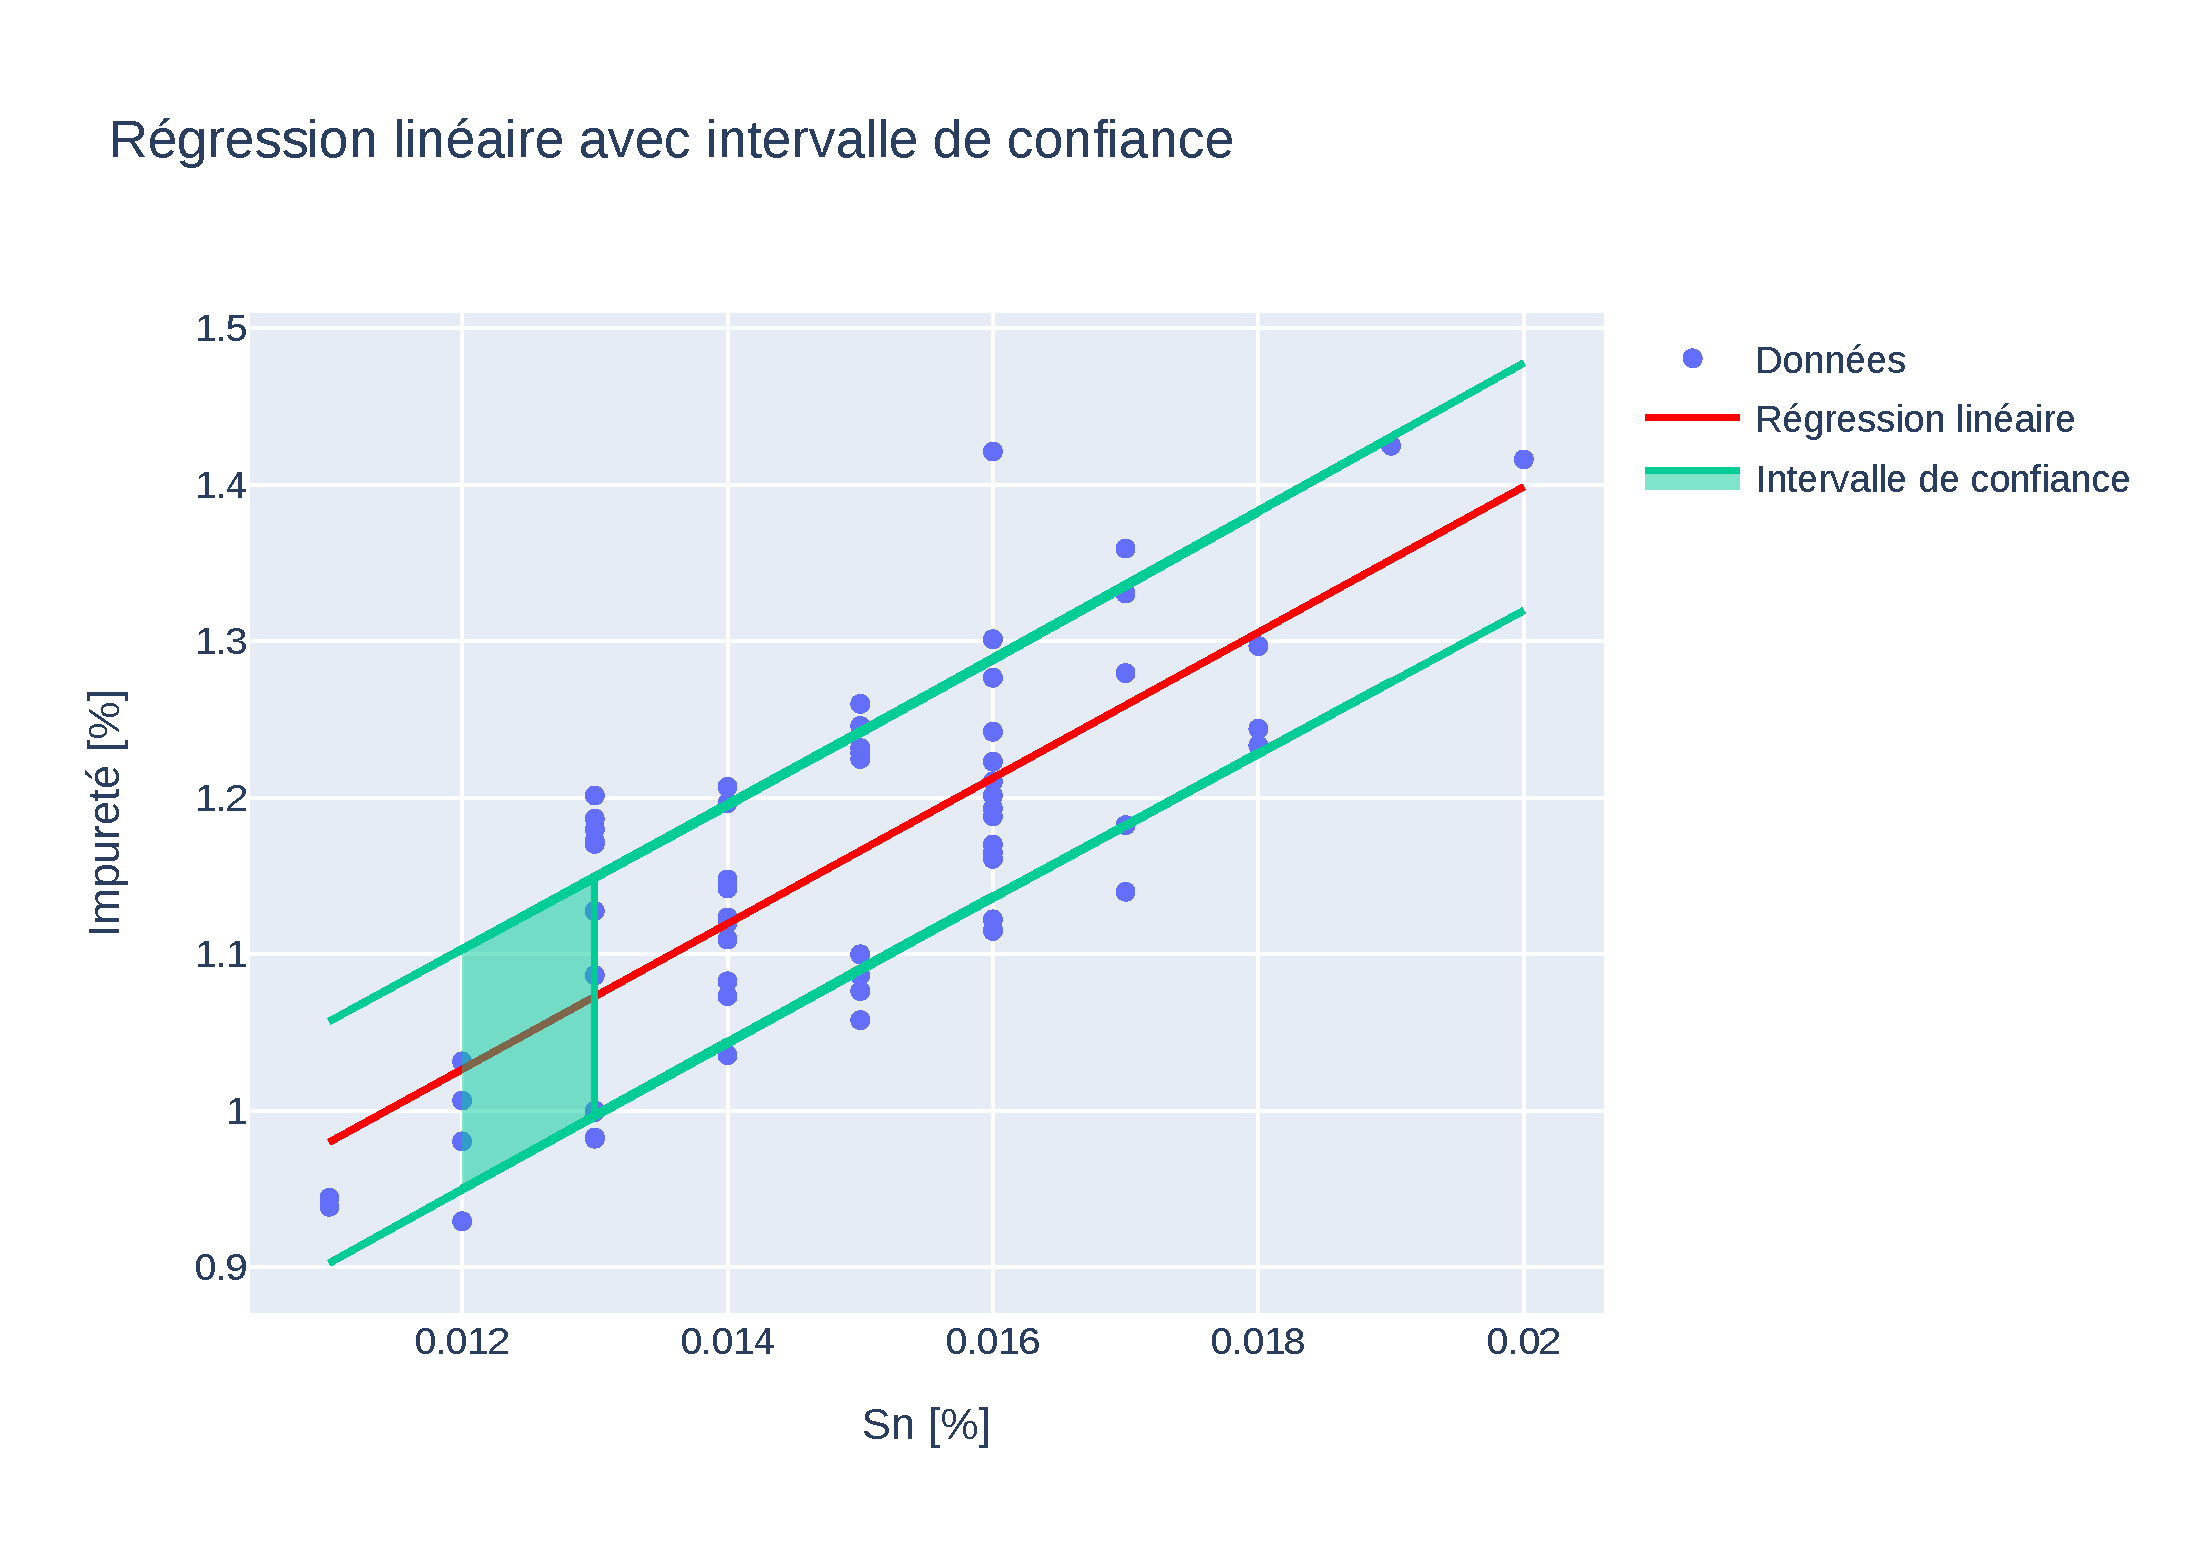
\includegraphics[width=\textwidth]{Figures/Regression_Impurete_Sn.pdf} 
  \end{column}
  \begin{column}{0.5\textwidth}
    \centering
    \textbf{L'impurété en fonction du cuivre (Cu)} \\
    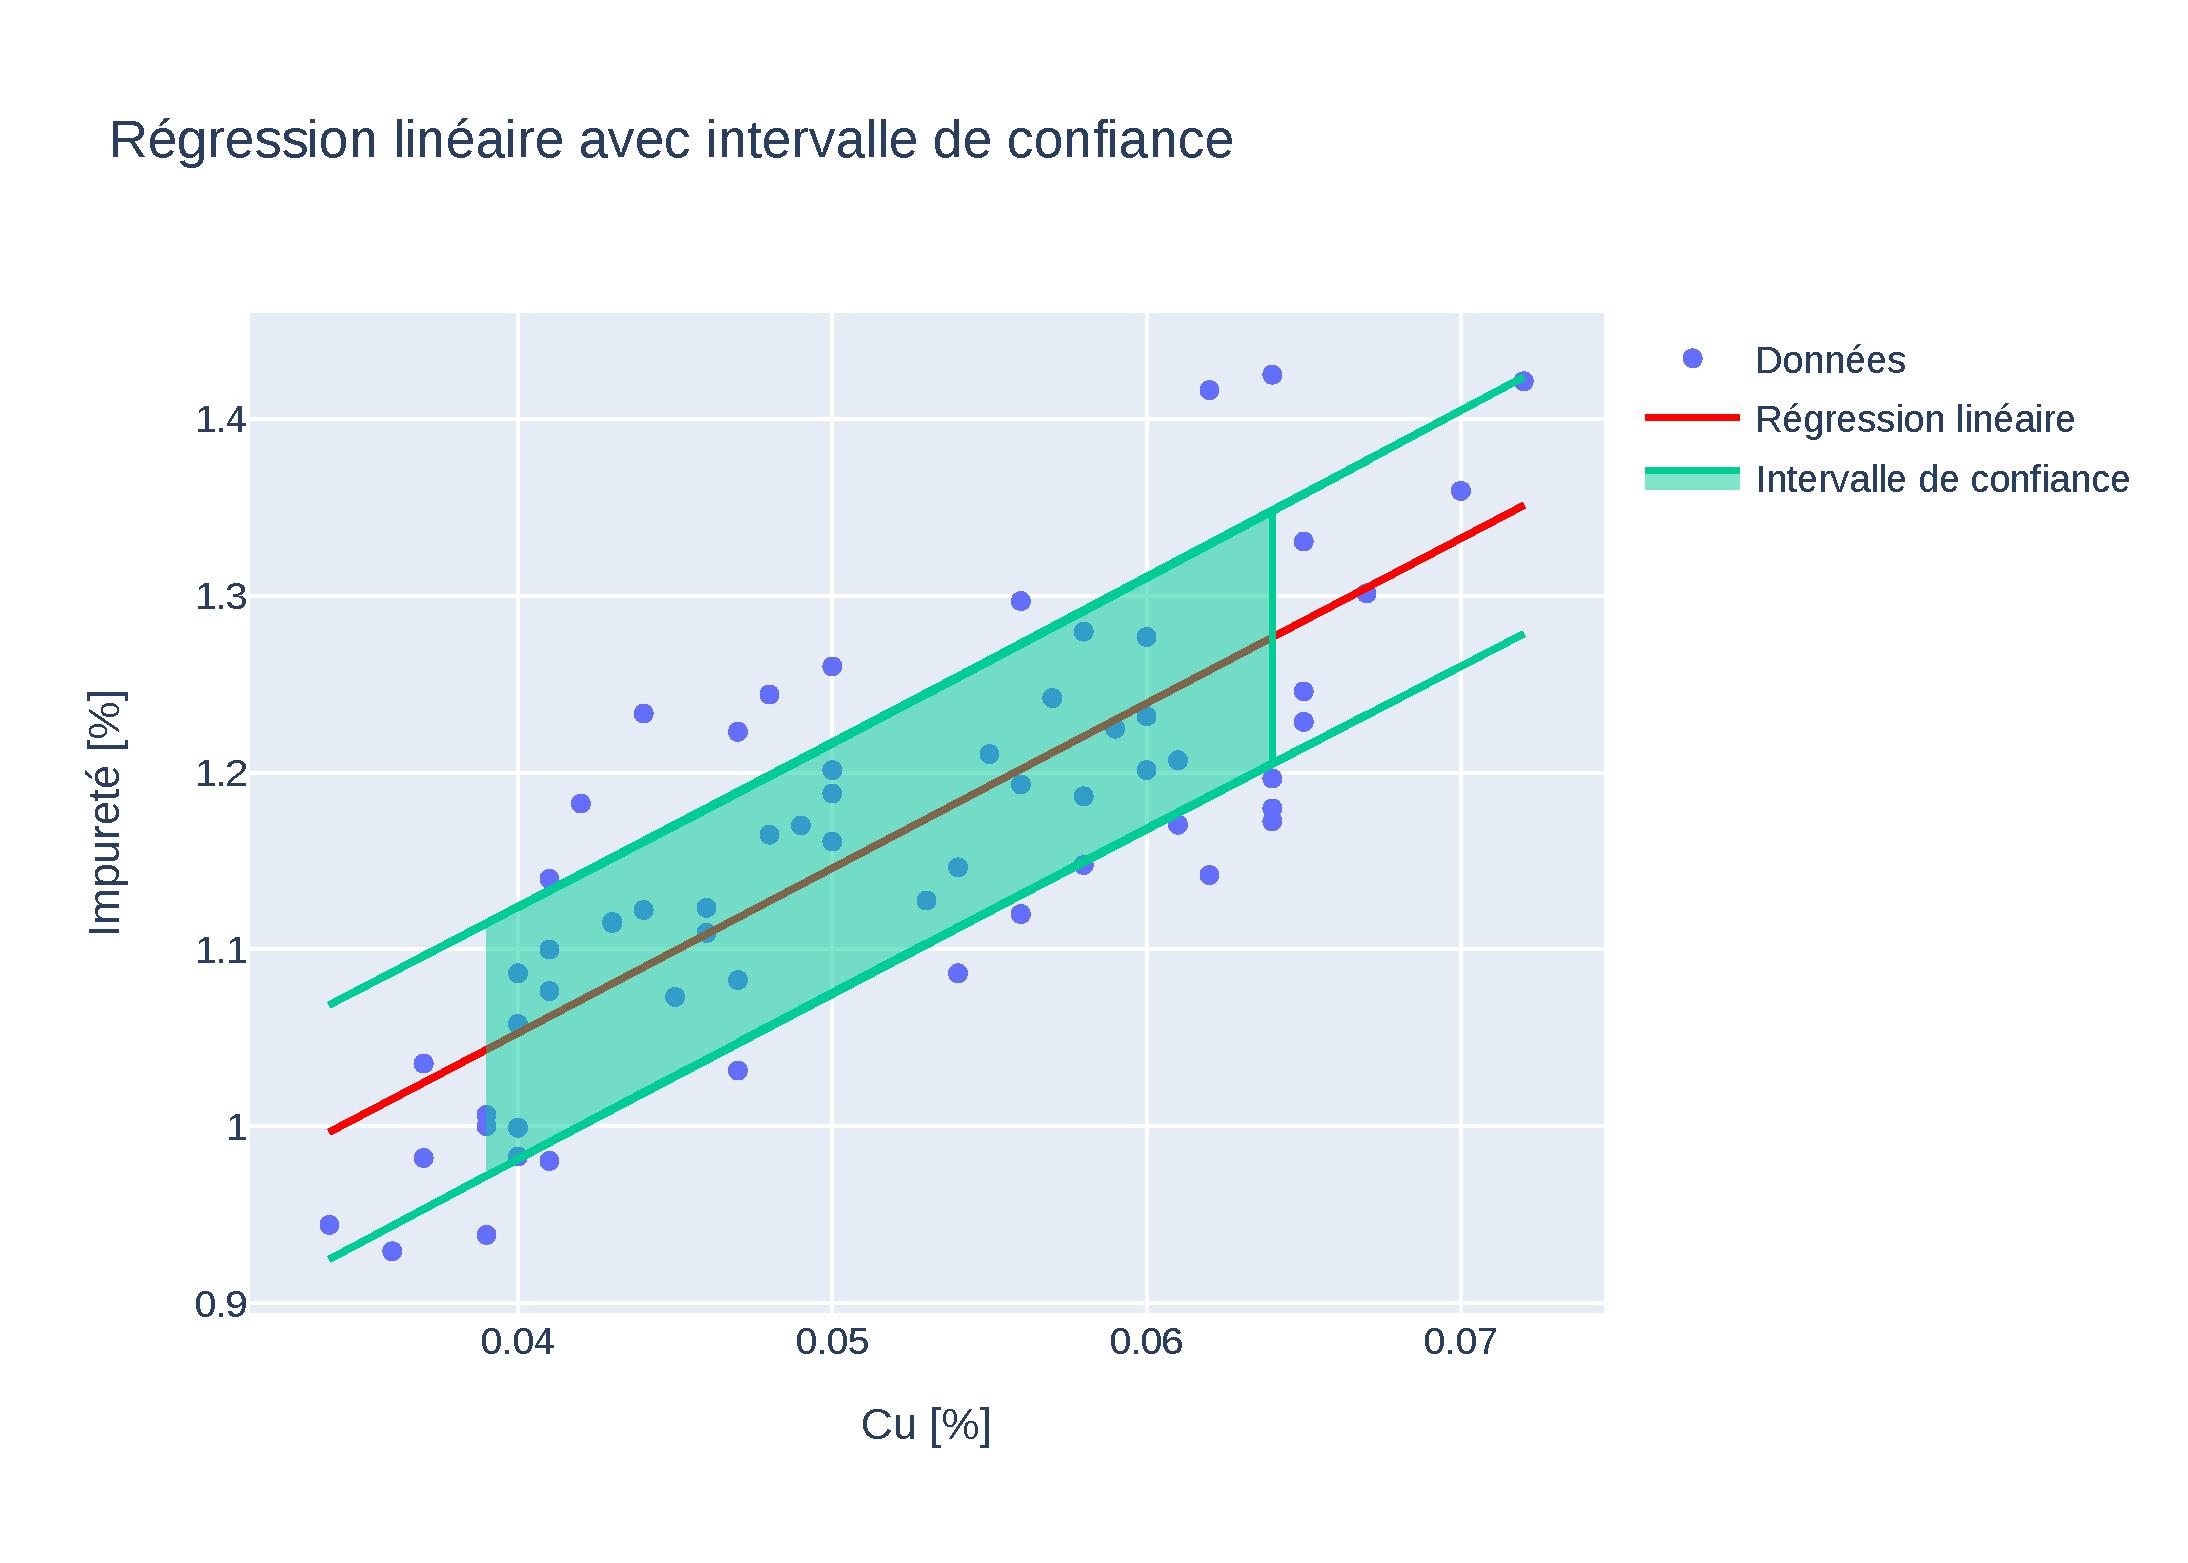
\includegraphics[width=\textwidth]{Figures/Regression_Impurete_Cu.pdf} 
  \end{column}
\end{columns}
\end{frame}


% Purete ONO
\begin{frame}
\frametitle{Ono}
\begin{columns}[t]
  \begin{column}{0.5\textwidth}
    \centering
    \textbf{La pureté Ono en fonction du cuivre (Cu)} \\
    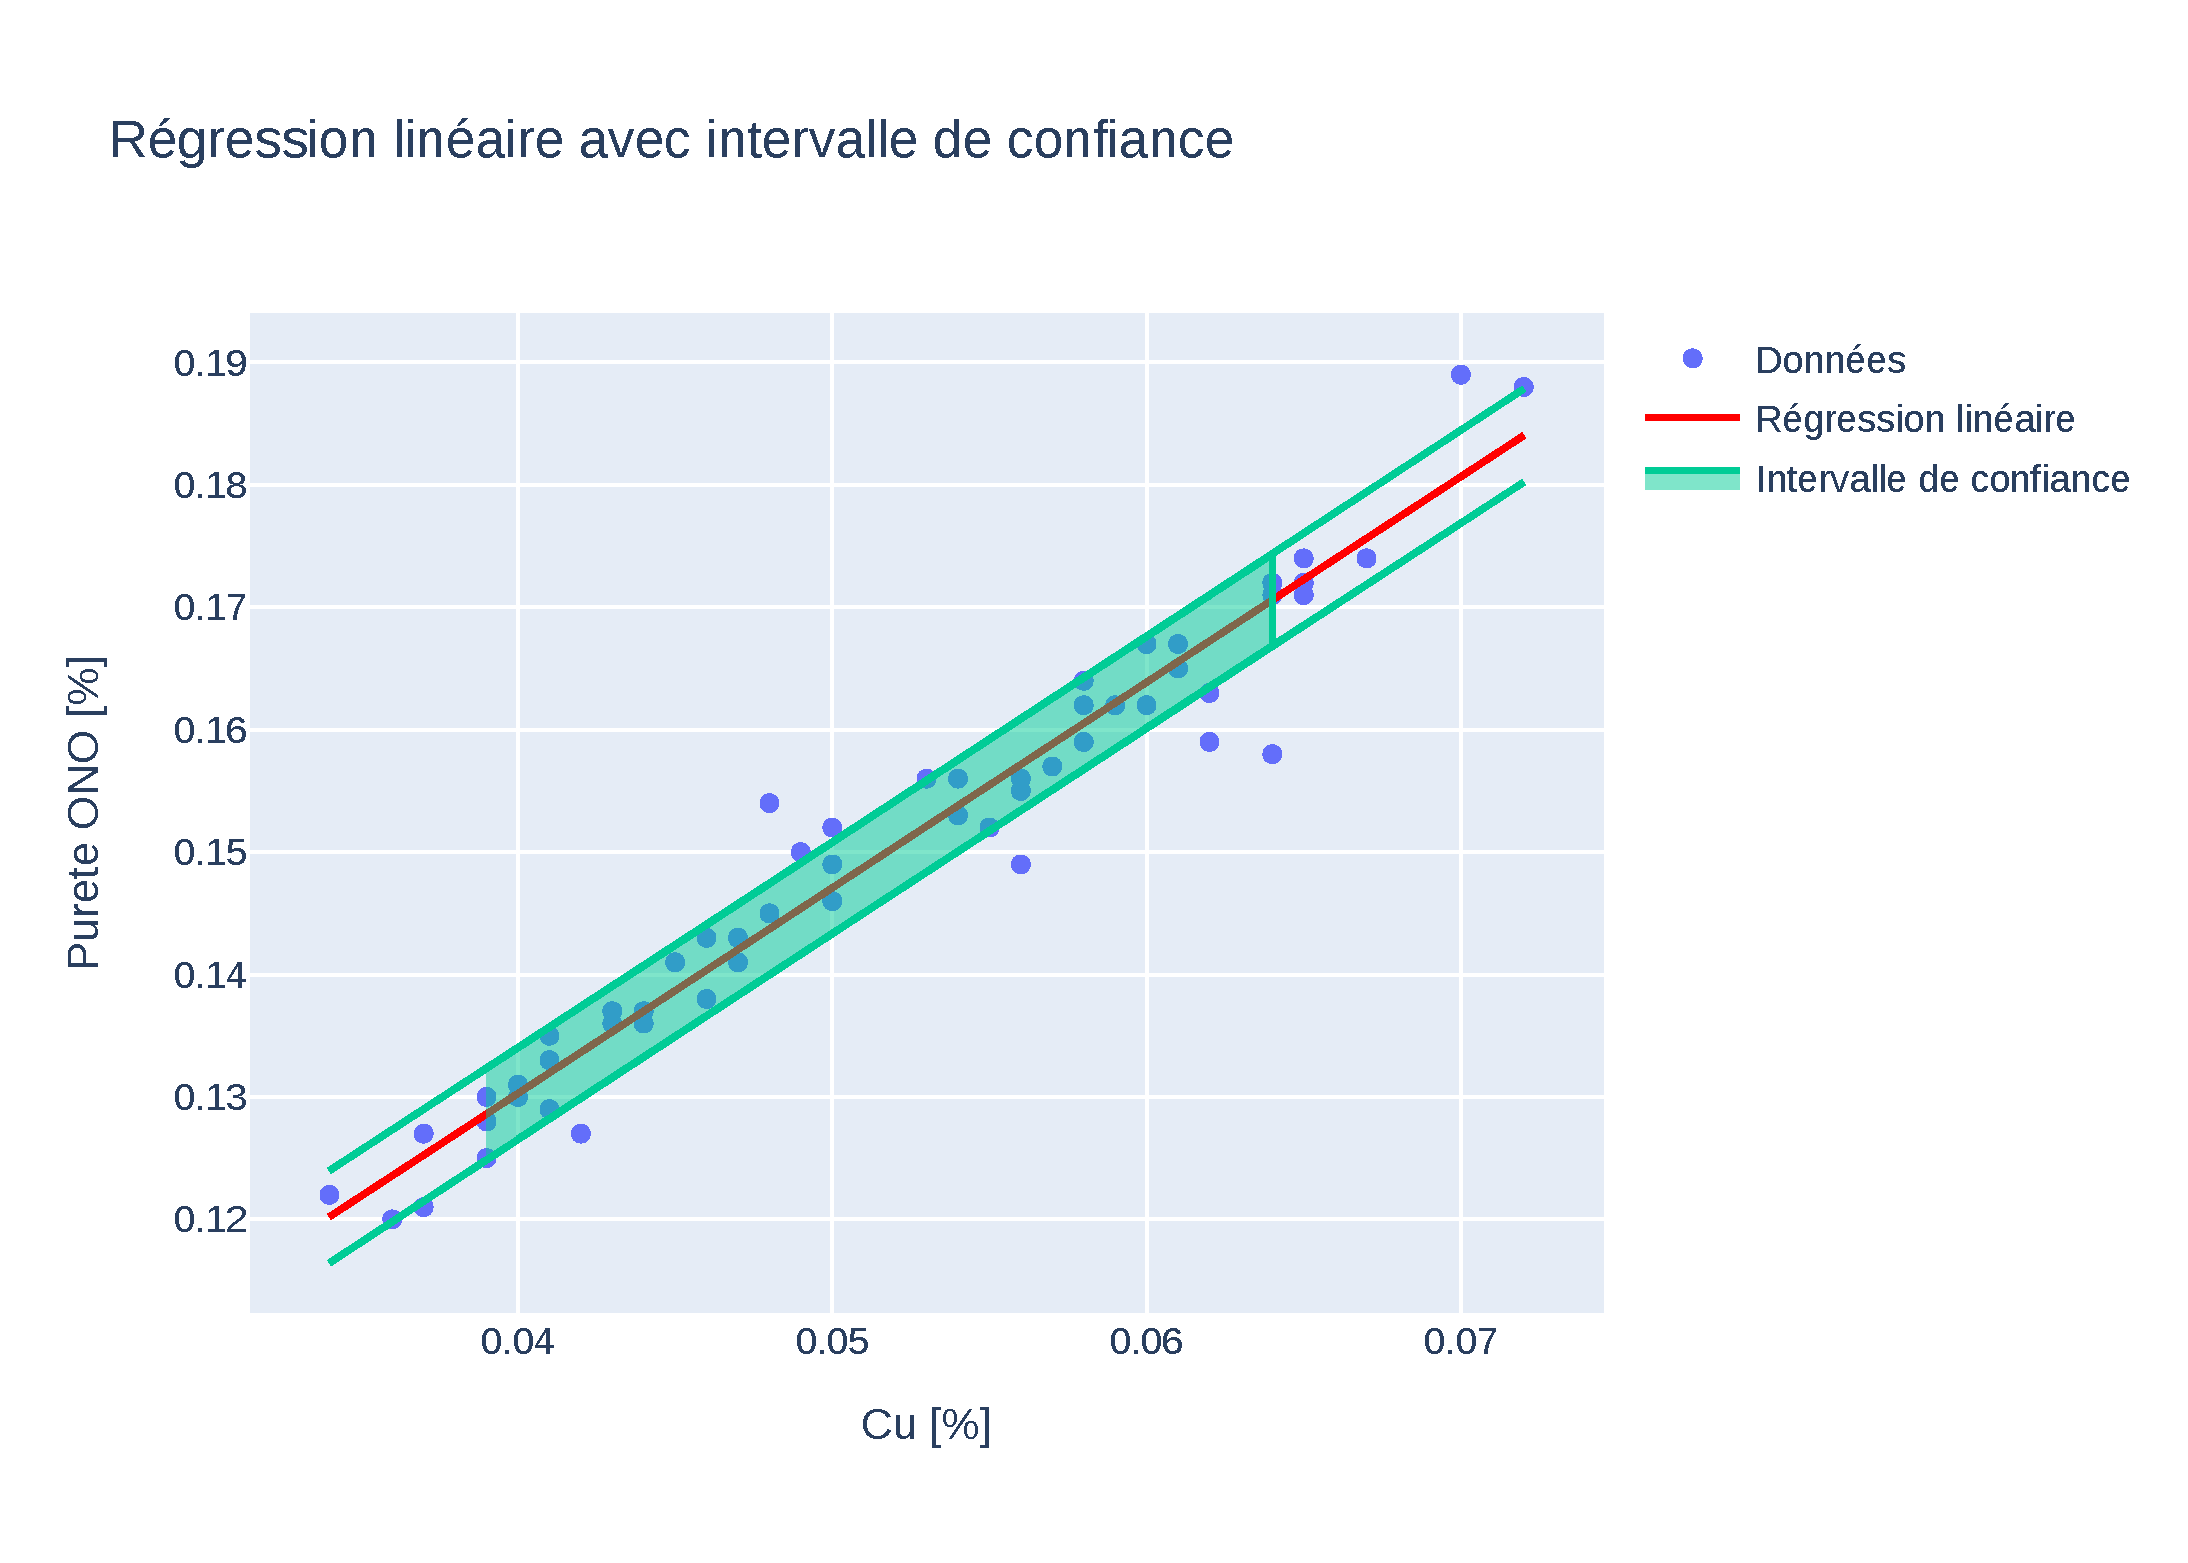
\includegraphics[width=\textwidth]{Figures/Regression_Ono_Cu.pdf} 
  \end{column}
  \begin{column}{0.5\textwidth}
    \centering
    \textbf{La pureté Ono en fonction du chrome (Cr)} \\
    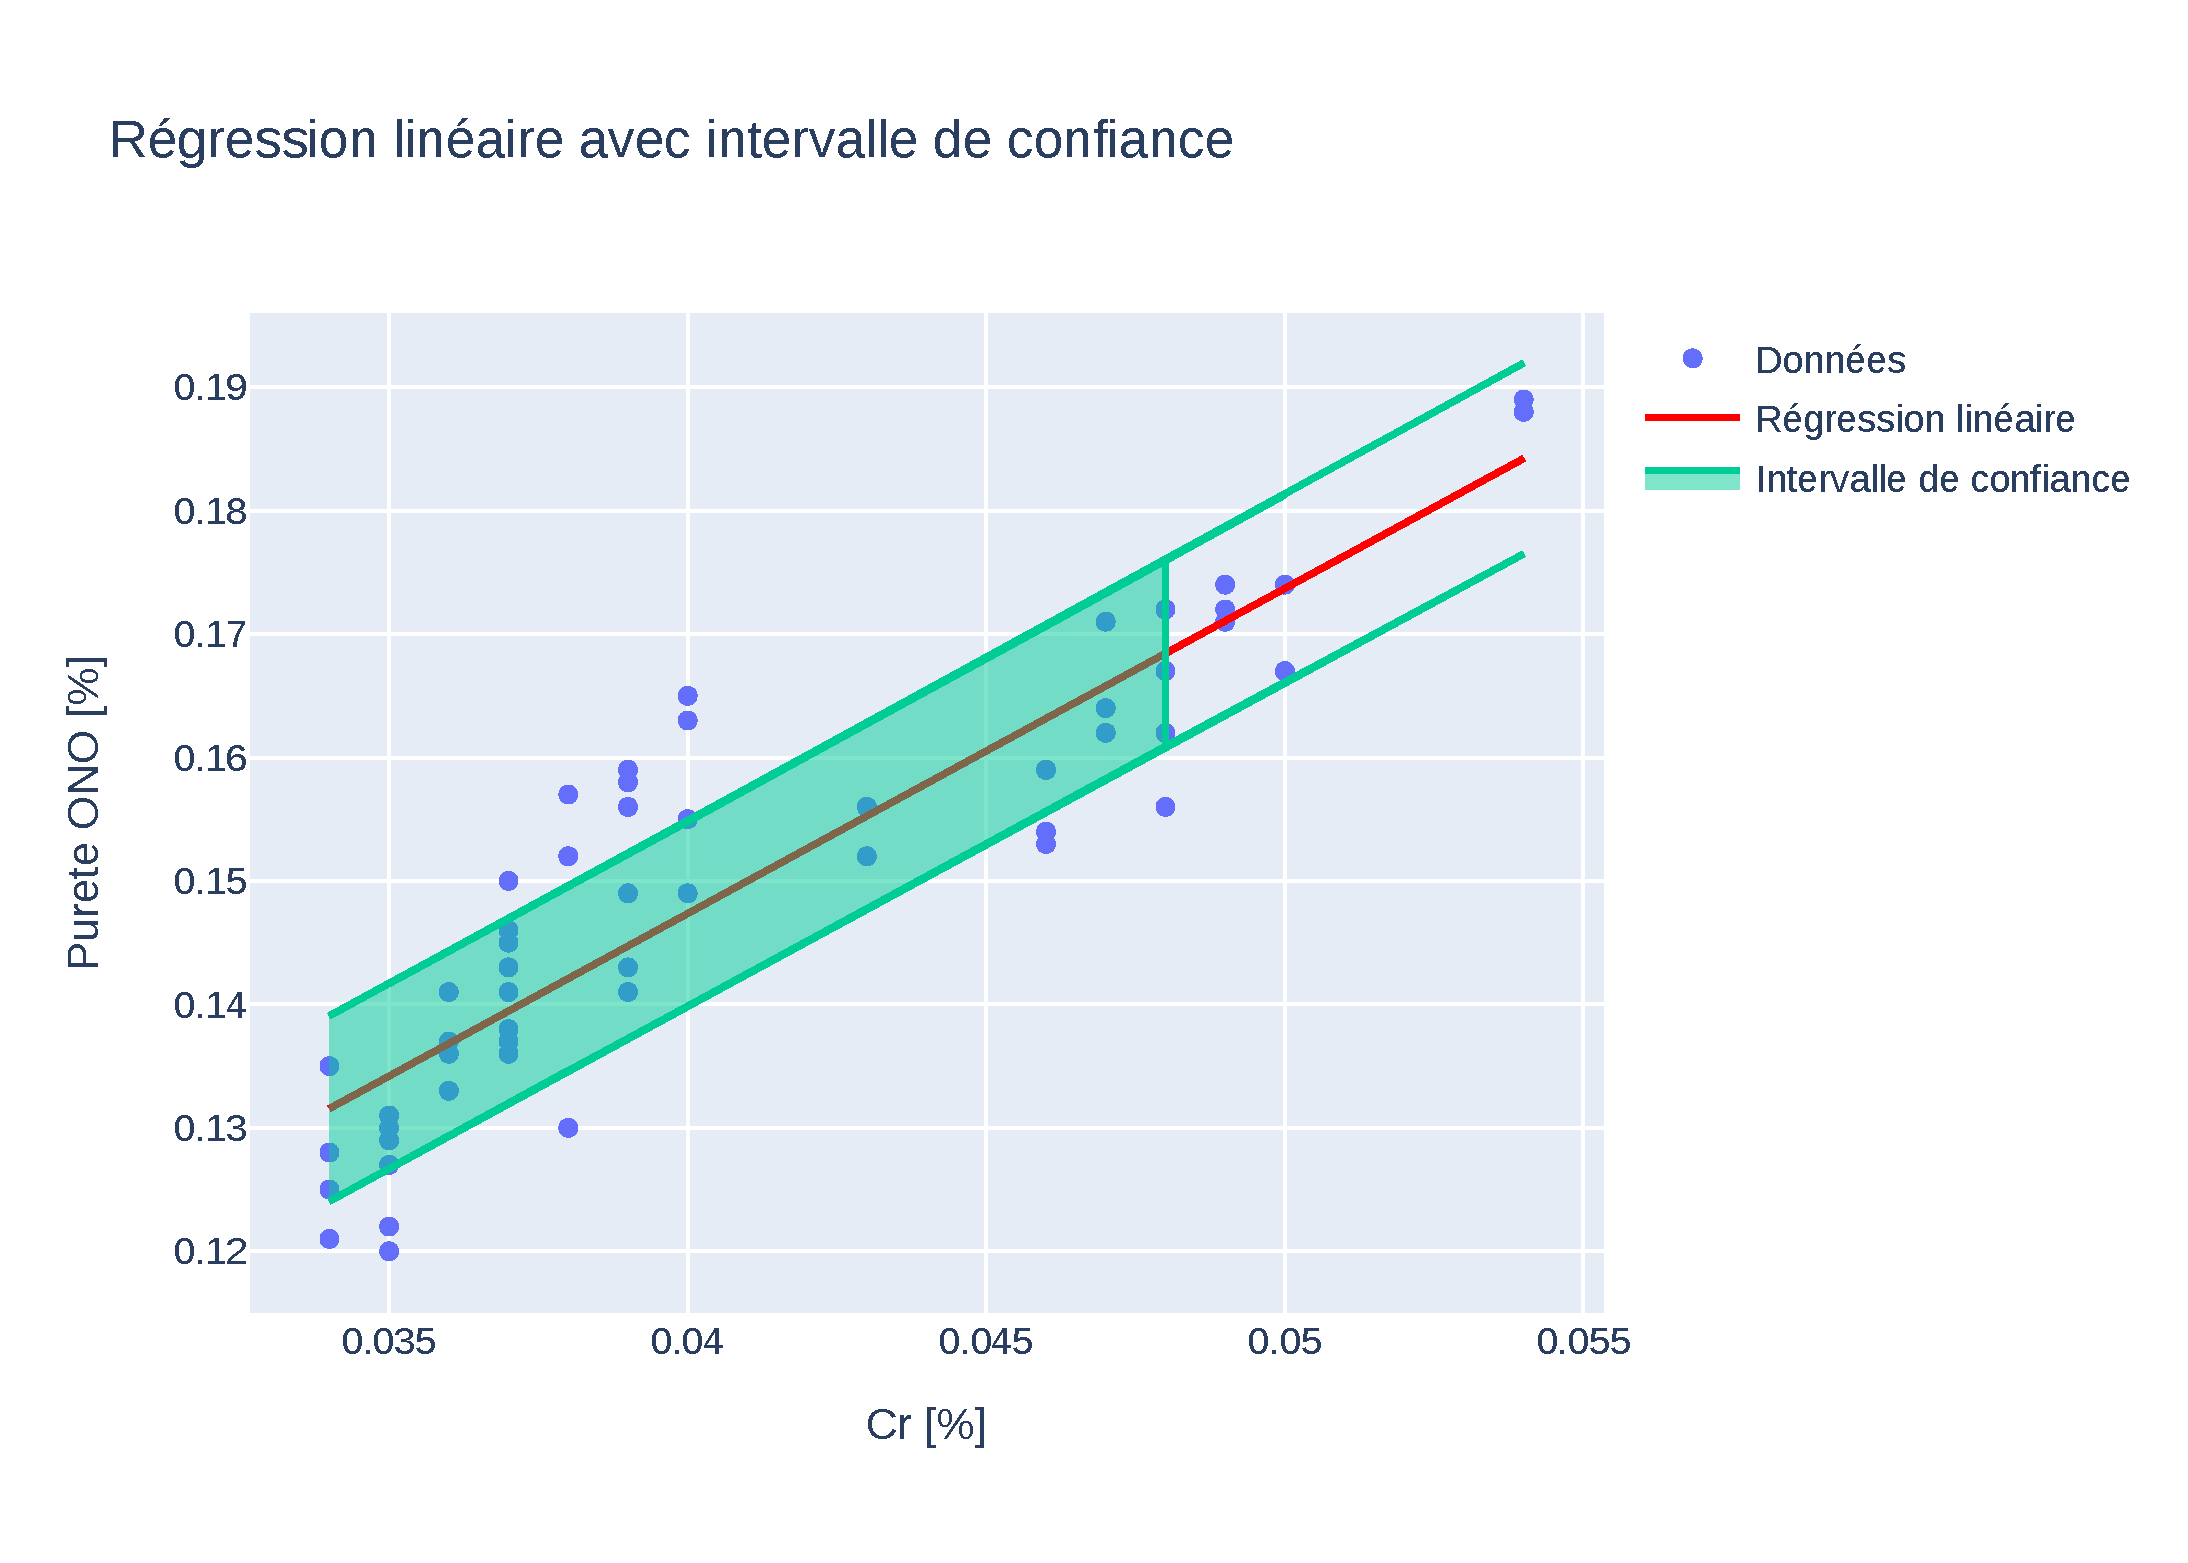
\includegraphics[width=\textwidth]{Figures/Regression_Ono_Cr.pdf} 
  \end{column}
\end{columns}
\end{frame}


% Ferrite
\begin{frame}
\frametitle{Ferrite}
\begin{columns}[t]
  \begin{column}{0.5\textwidth}
    \centering
    \textbf{La Ferrite en fonction du cuivre (Cu)} \\
    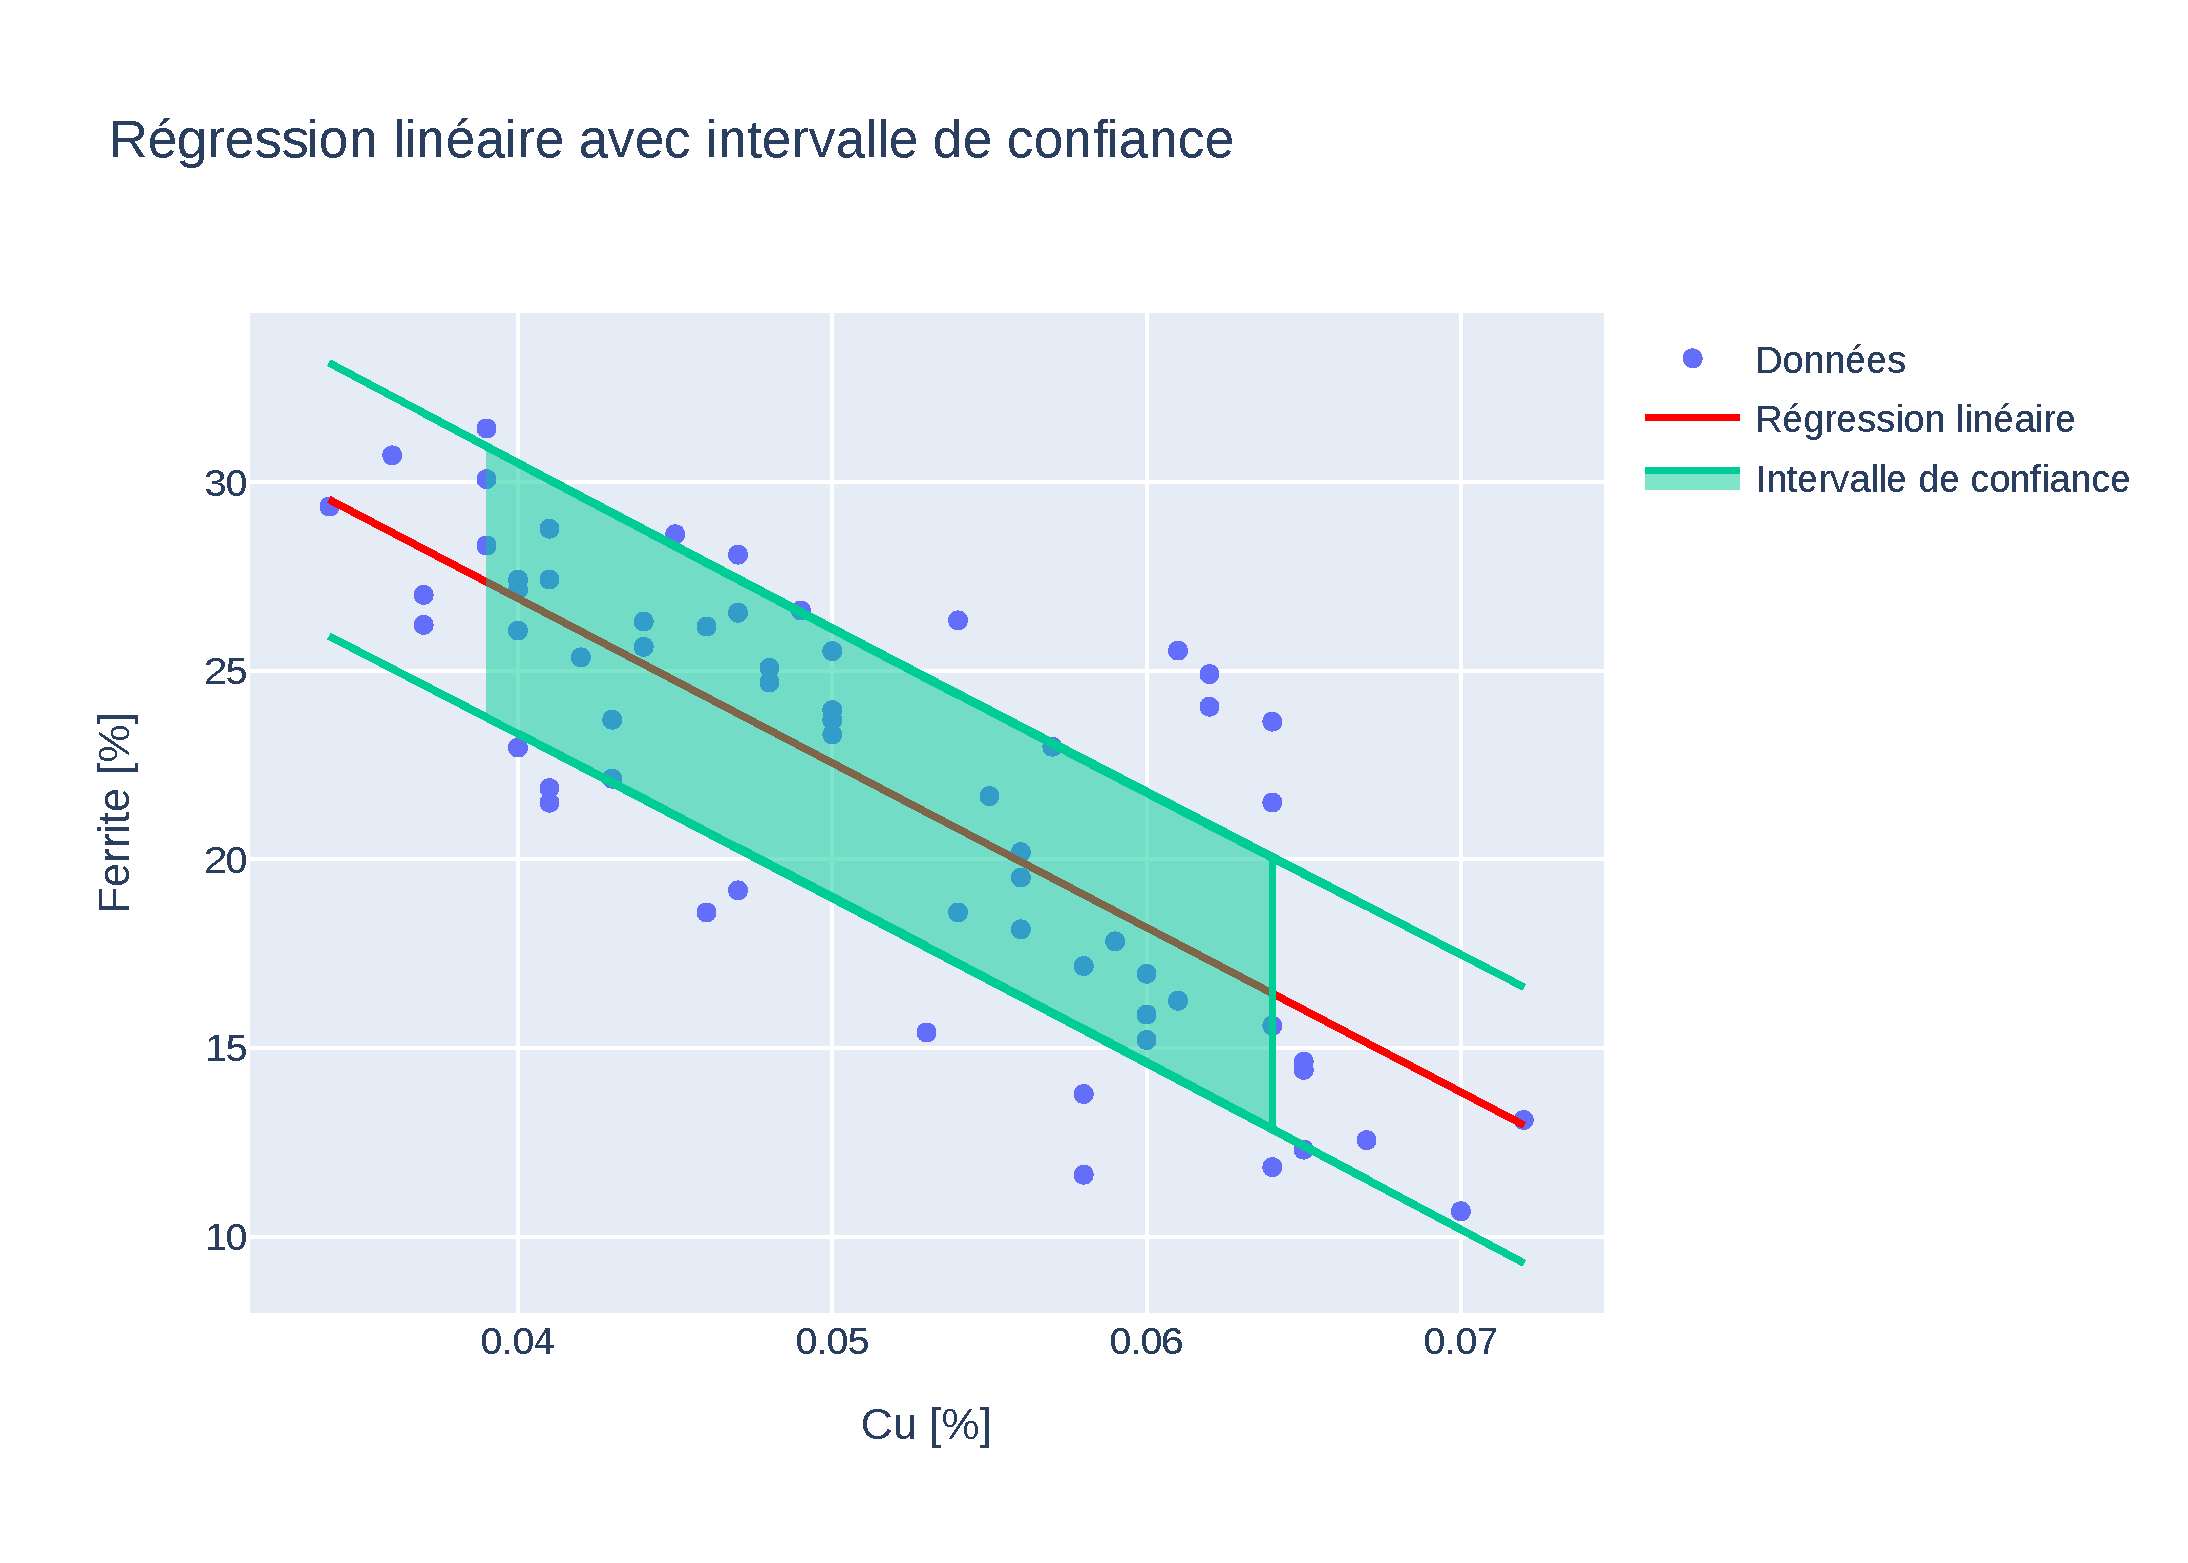
\includegraphics[width=\textwidth]{Figures/Regression_Ferrite_Cu.pdf} 
  \end{column}
  \begin{column}{0.5\textwidth}
    \centering
    \textbf{La Ferrite en fonction de l'ntimoine Sb} \\
    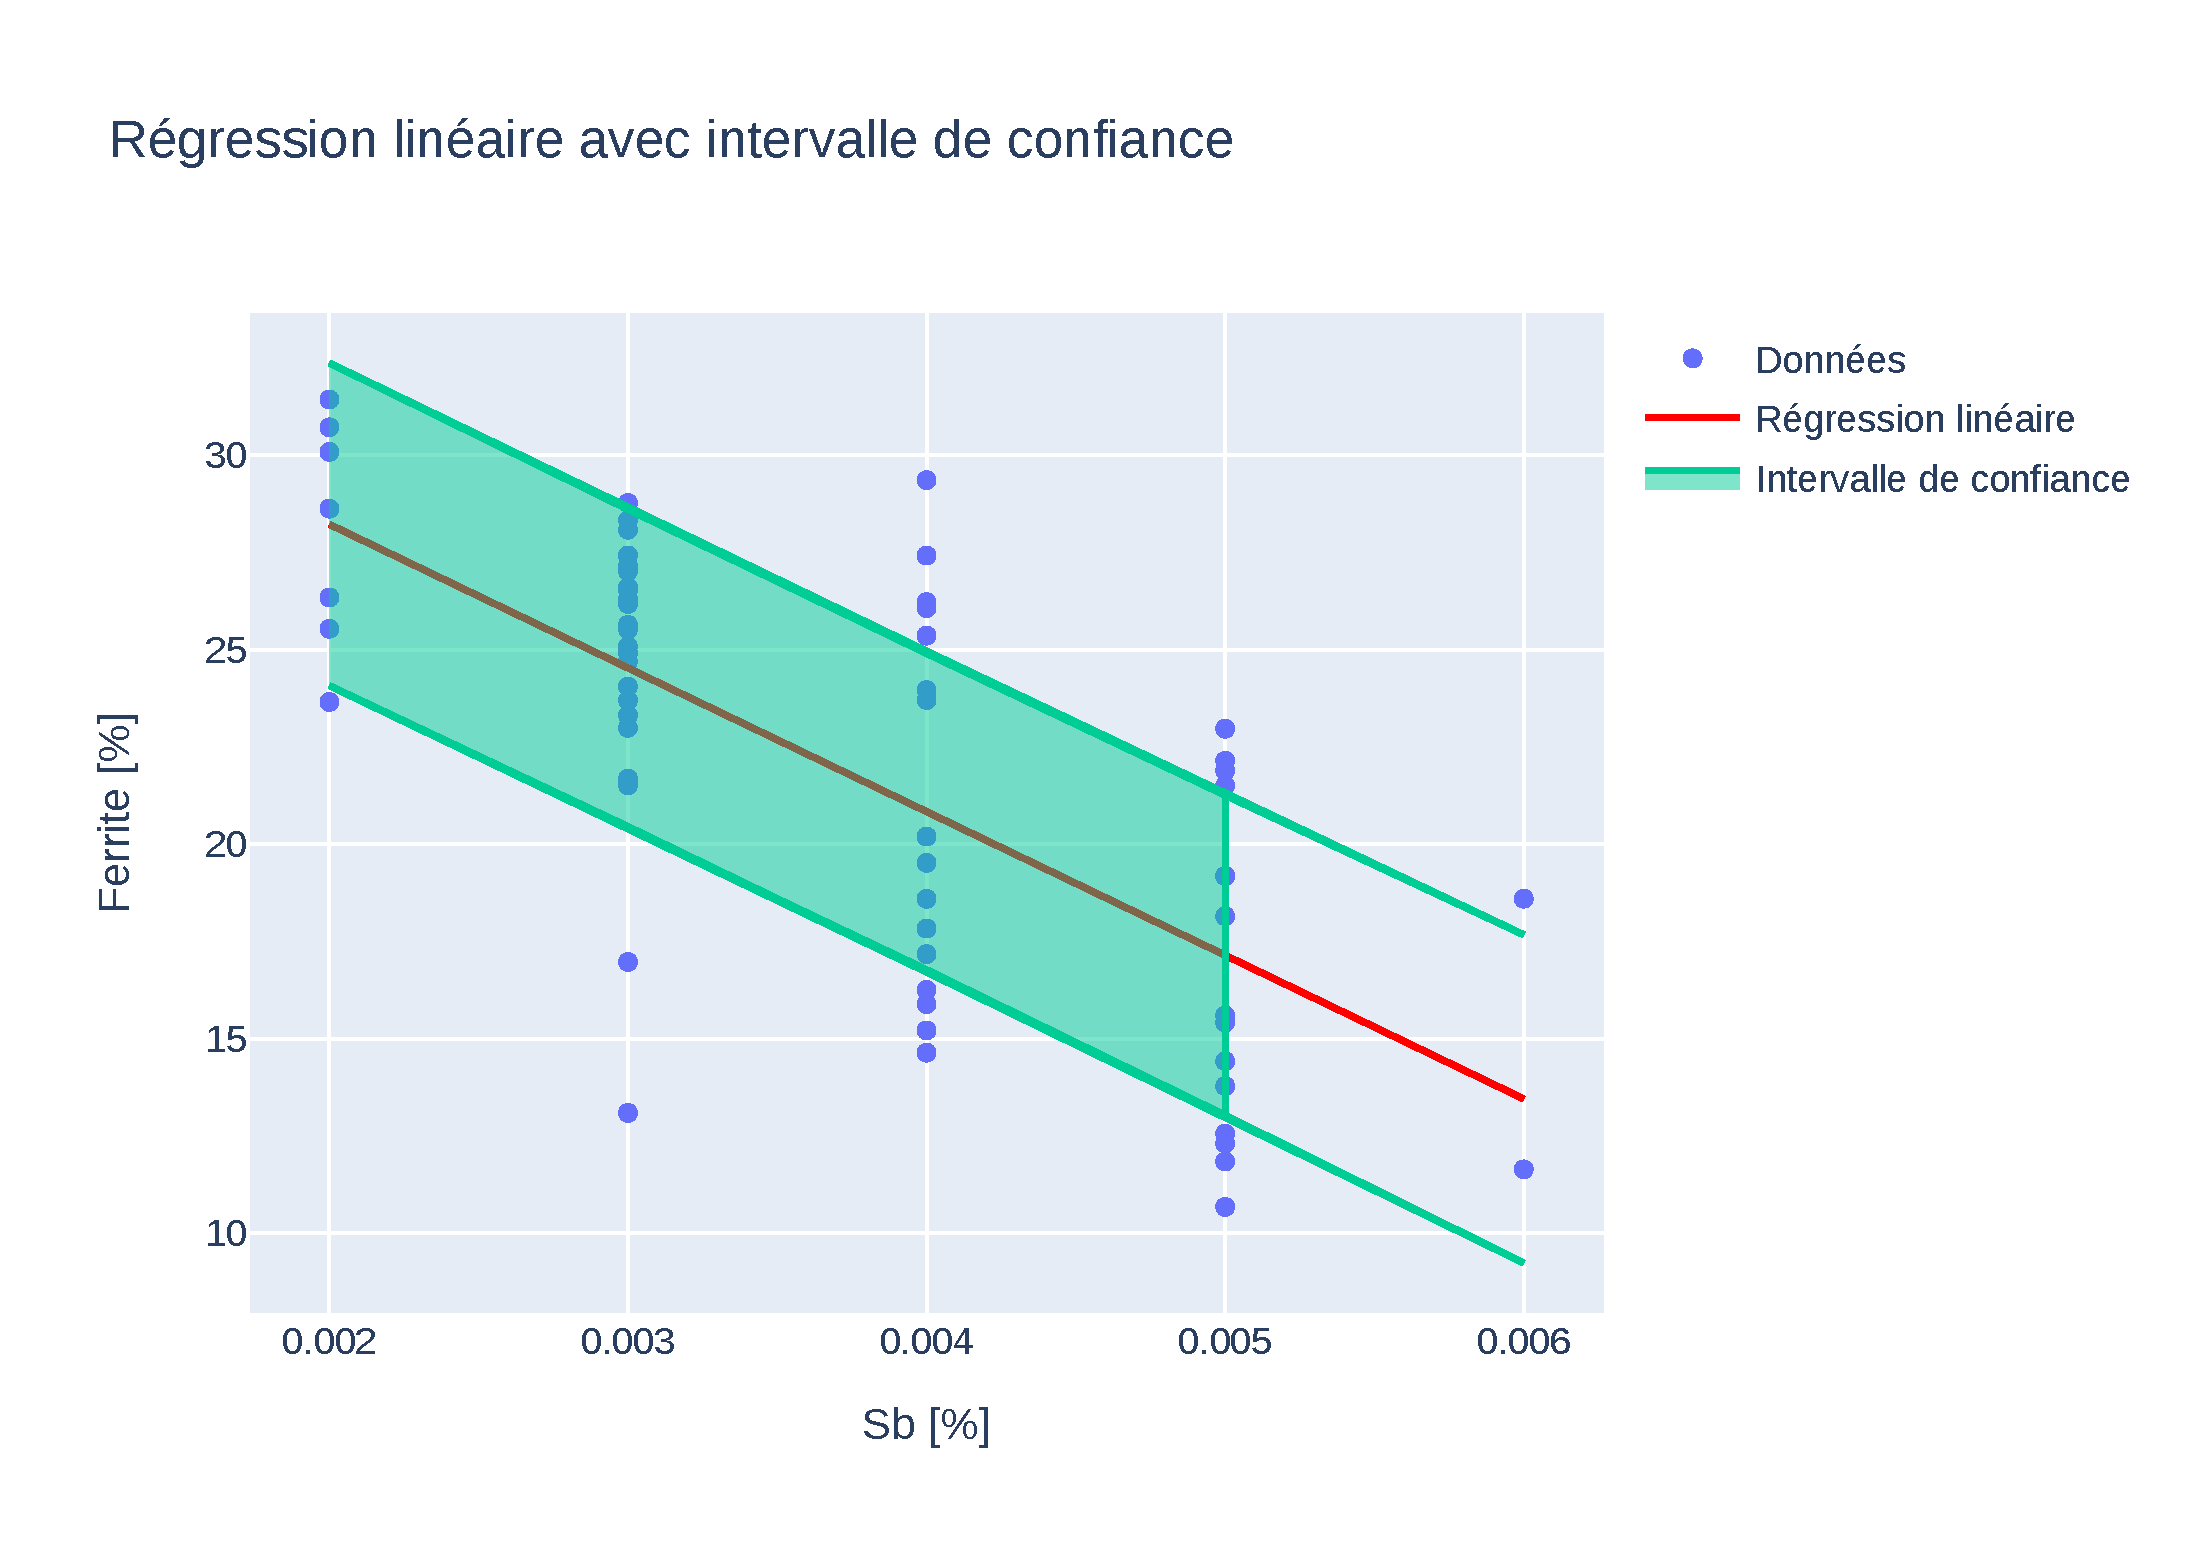
\includegraphics[width=\textwidth]{Figures/Regression_Ferrite_Sb.pdf} 
  \end{column}
\end{columns}
\end{frame}



% Rm
\begin{frame}
\frametitle{Rm}
\begin{columns}[t]
  \begin{column}{0.5\textwidth}
    \centering
    \textbf{La Résistance mécanique en fonction du Cuivre} \\
    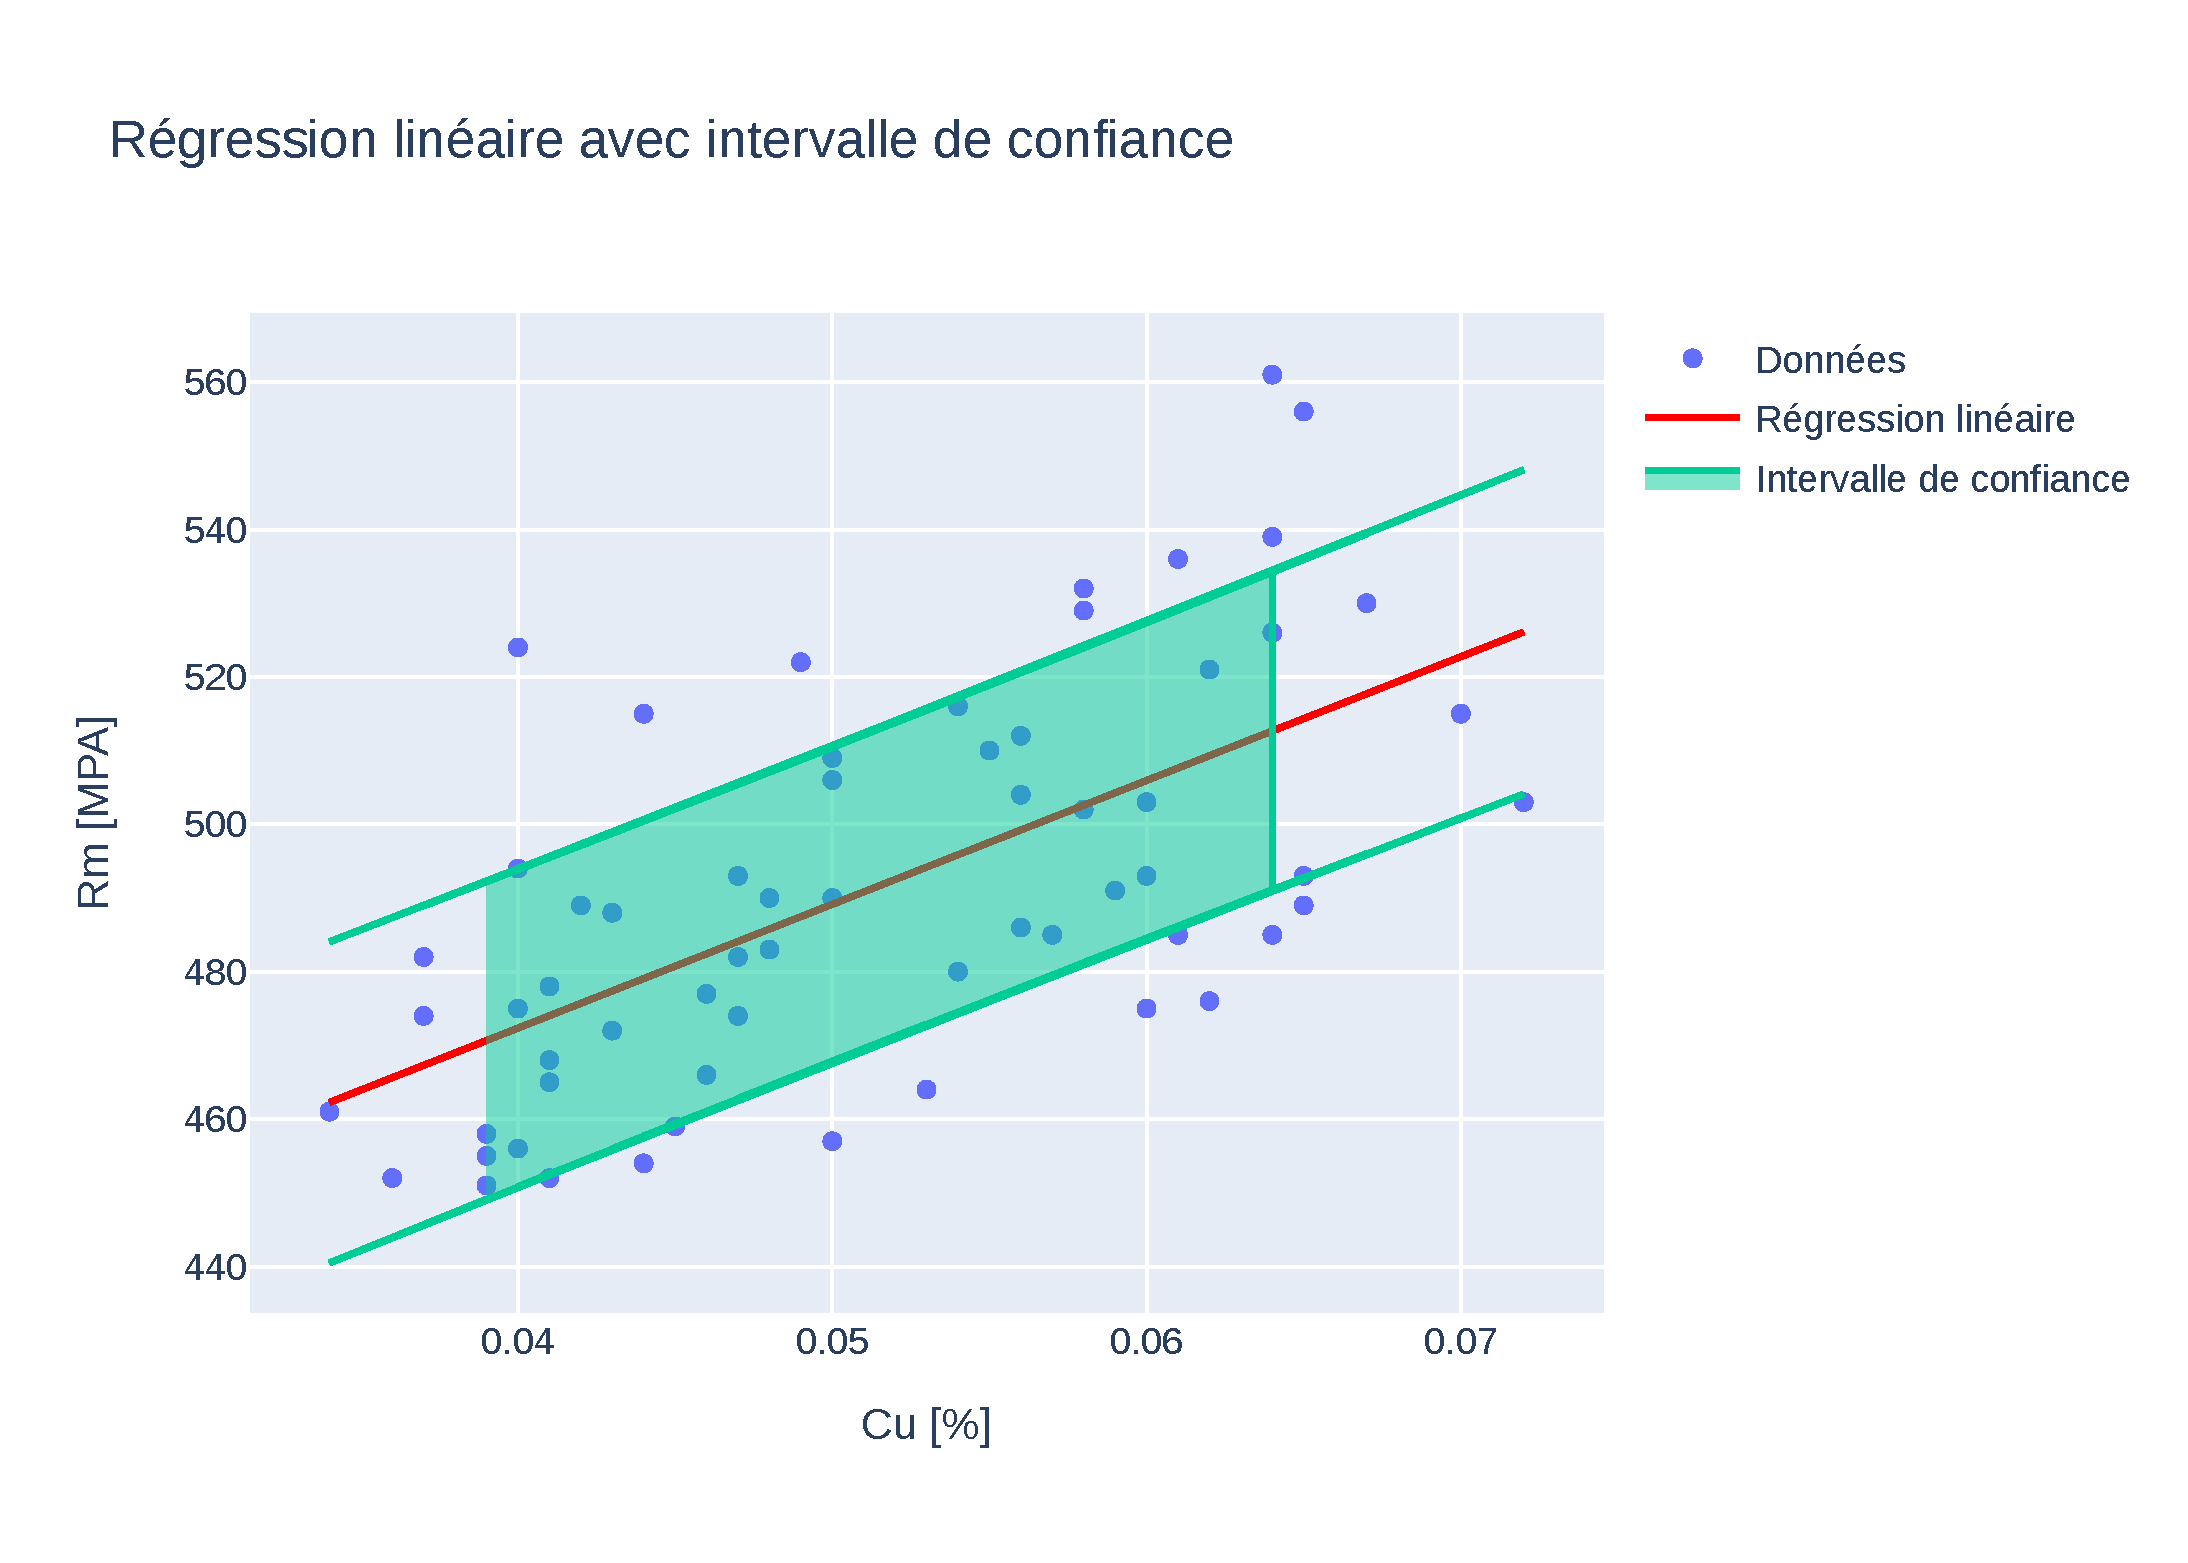
\includegraphics[width=\textwidth]{Figures/Regression_Cu_Rm.pdf} 
  \end{column}
  \begin{column}{0.5\textwidth}
    \centering
    \textbf{La Résistance mécanique en fonction du Sn} \\
    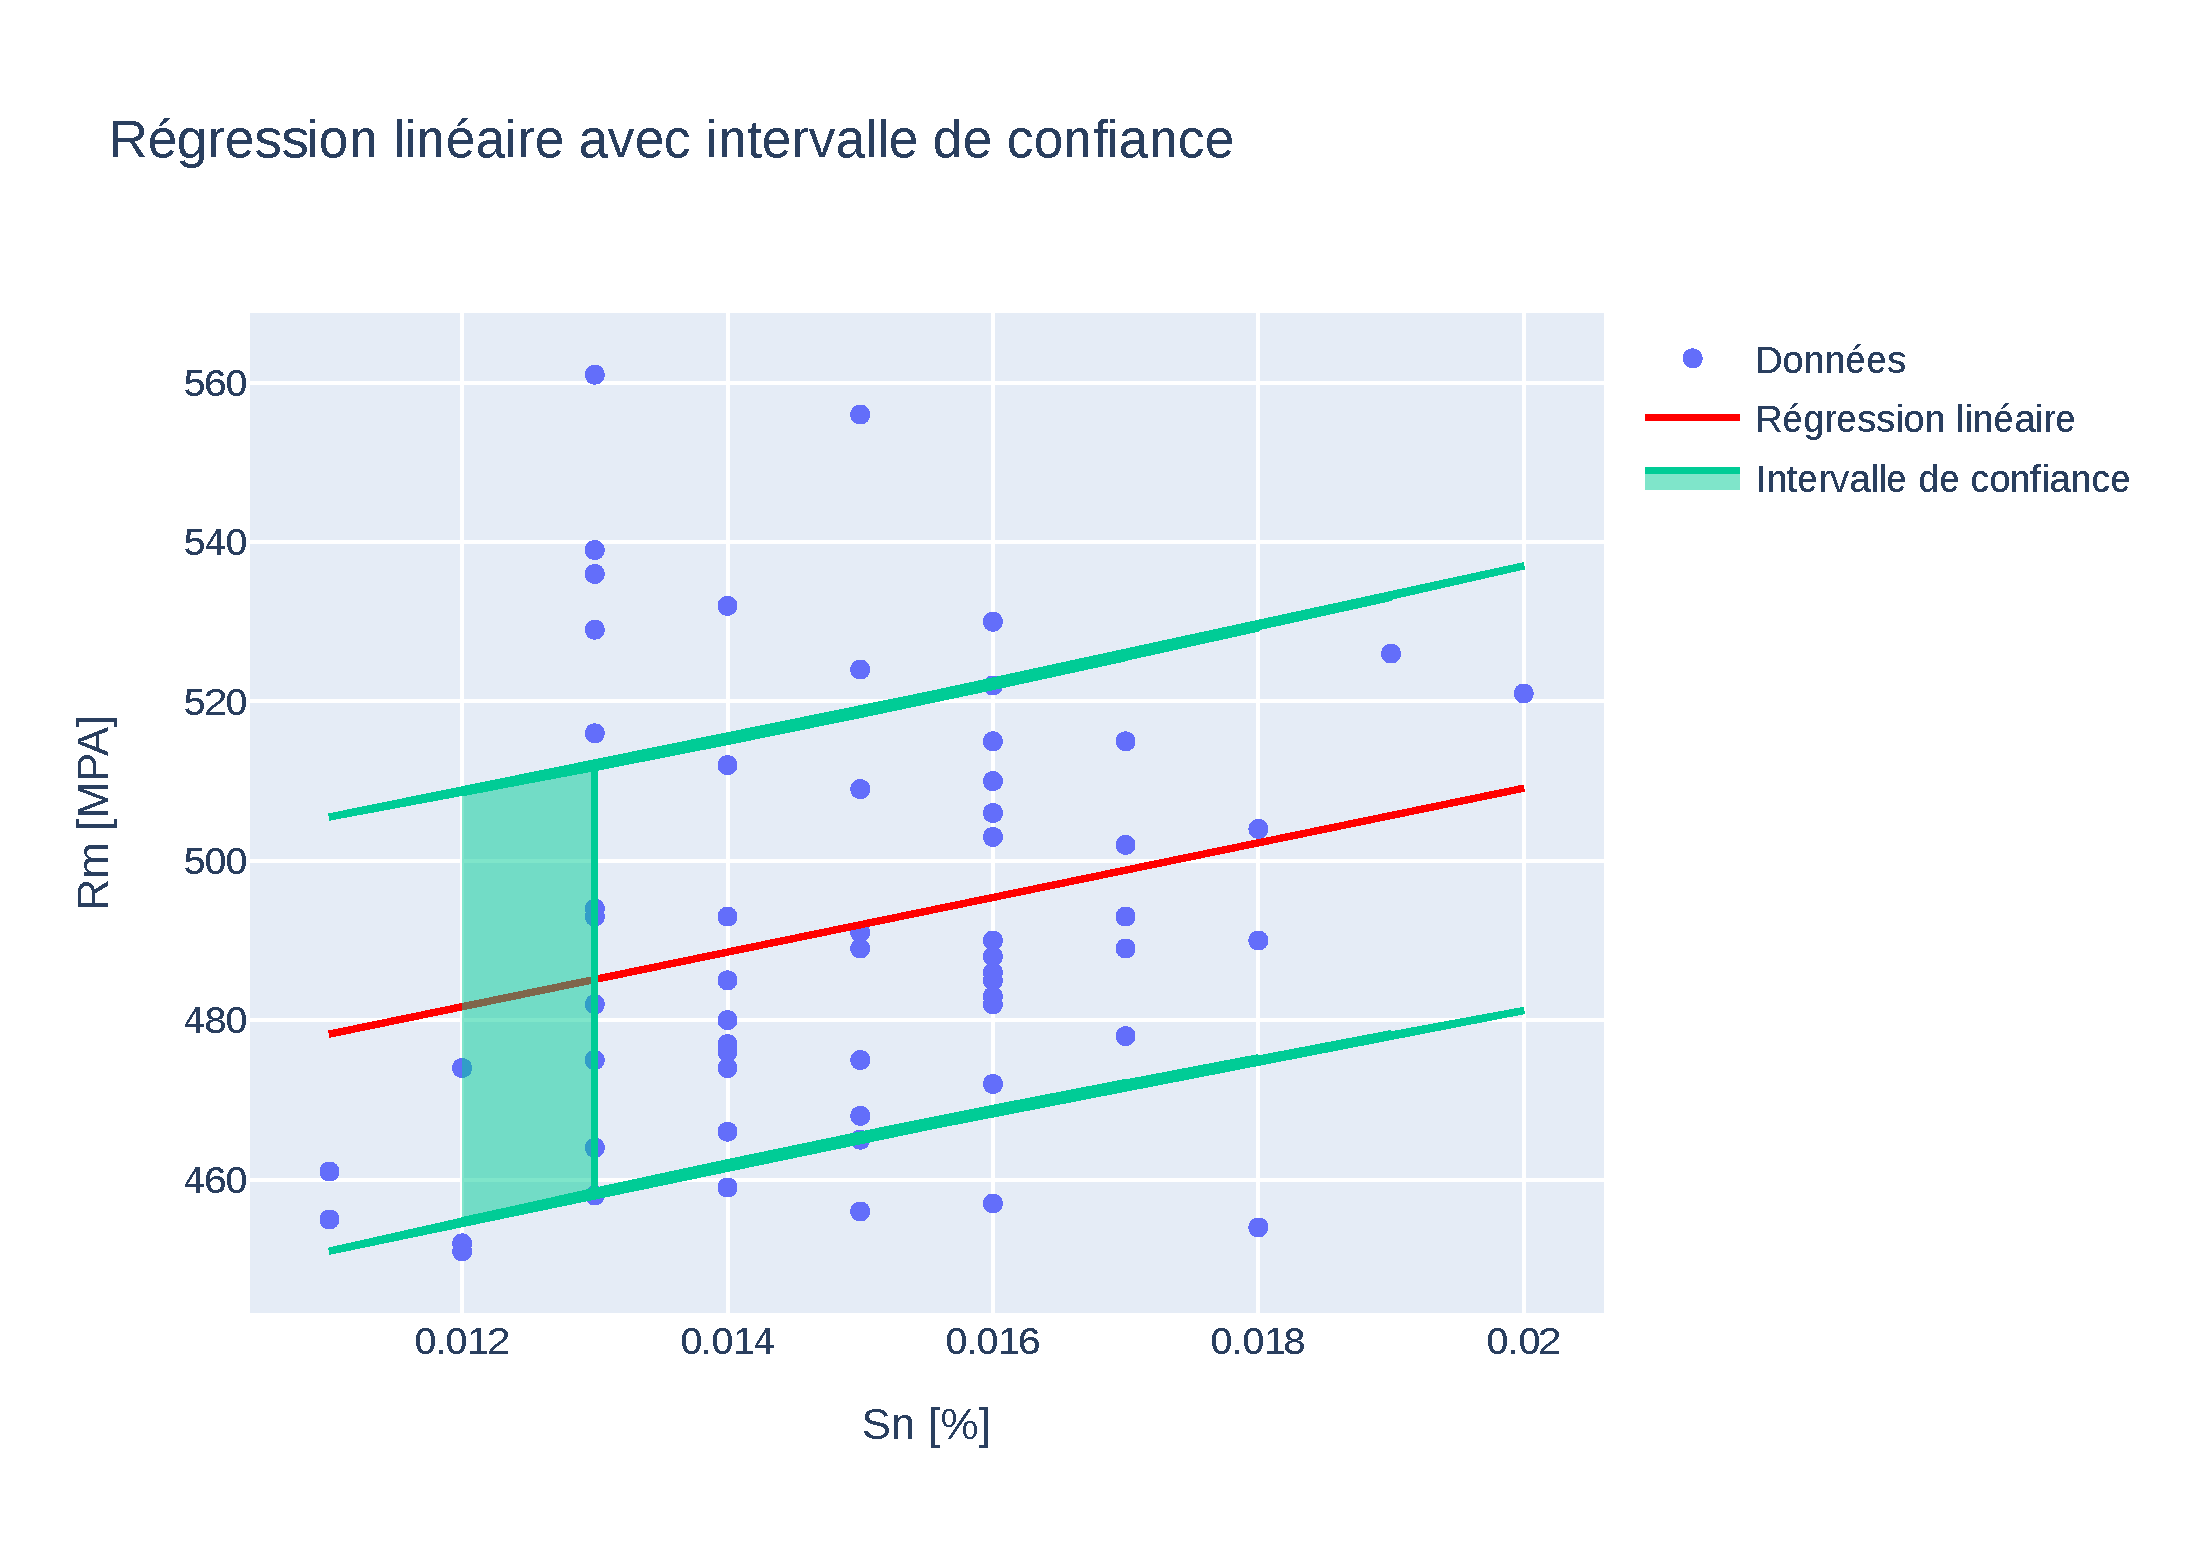
\includegraphics[width=\textwidth]{Figures/Regression_Sn_Rm.pdf} 
  \end{column}
\end{columns}
\end{frame}

% Allongement et Rm
\begin{frame}
\frametitle{Allongement et Rm}
\begin{columns}[t]
  \begin{column}{0.5\textwidth}
    \centering
    \textbf{La Résistance mécanique en fonction du Cr} \\
    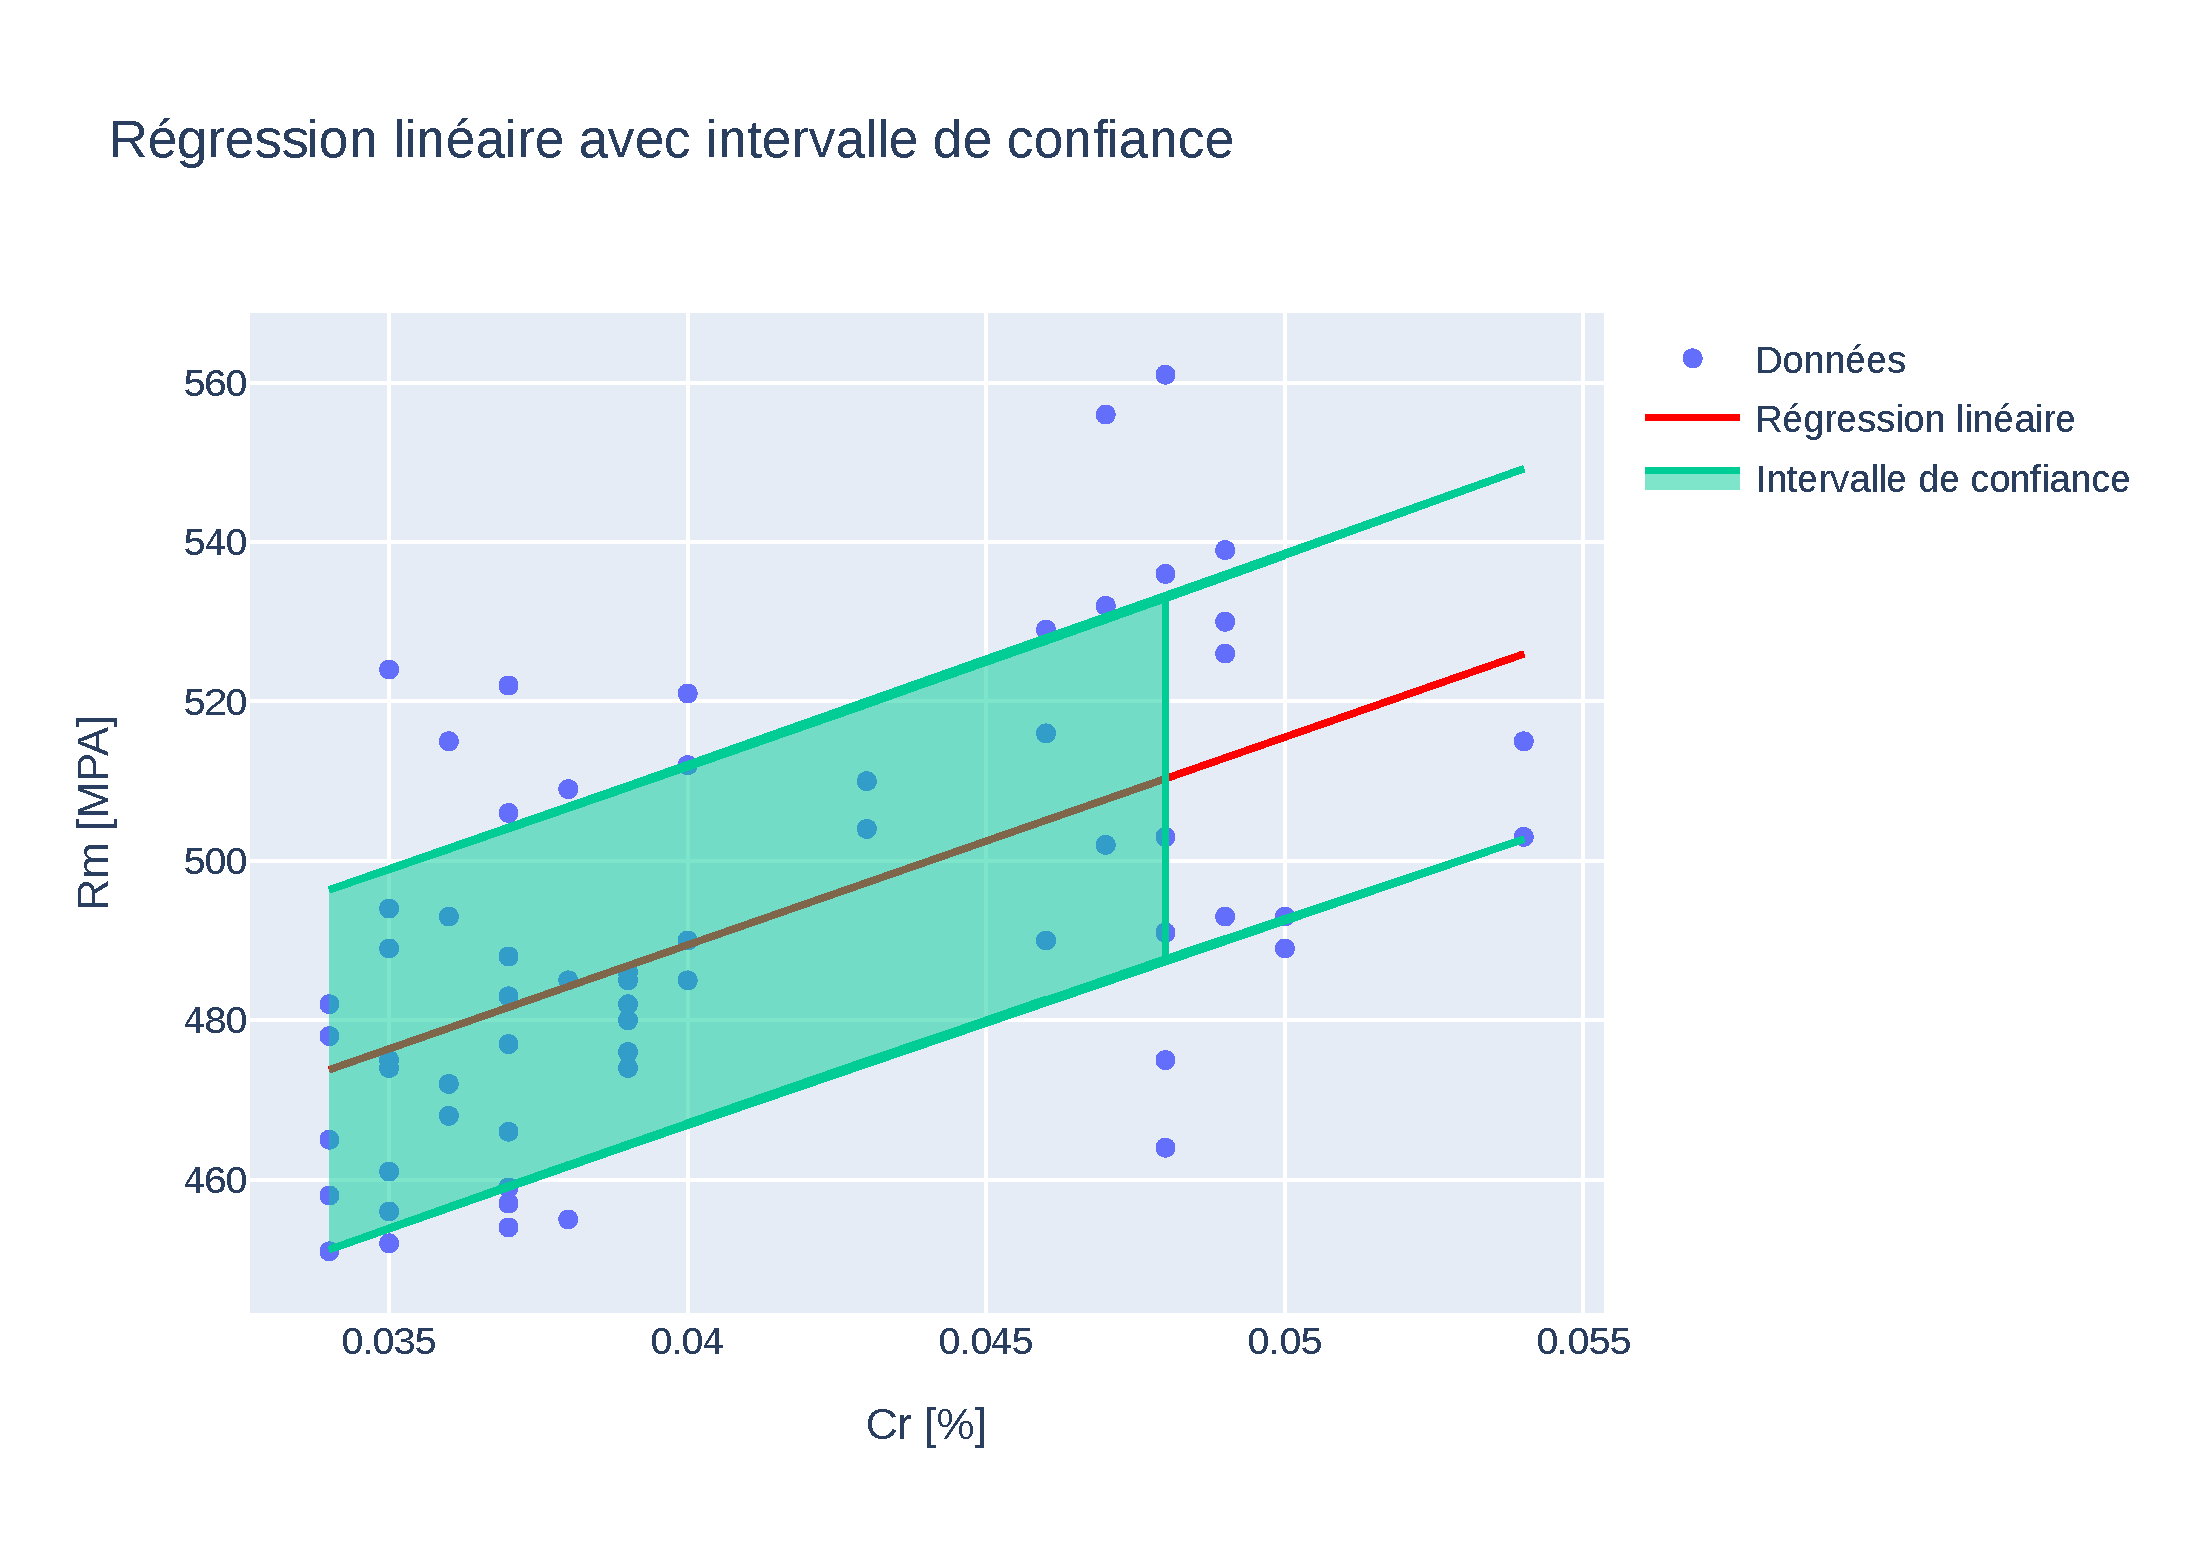
\includegraphics[width=\textwidth]{Figures/Regression_Cr_Rm.pdf} 
  \end{column}
  \begin{column}{0.5\textwidth}
    \centering
    \textbf{L'allongement en fonction du  Cr} \\
    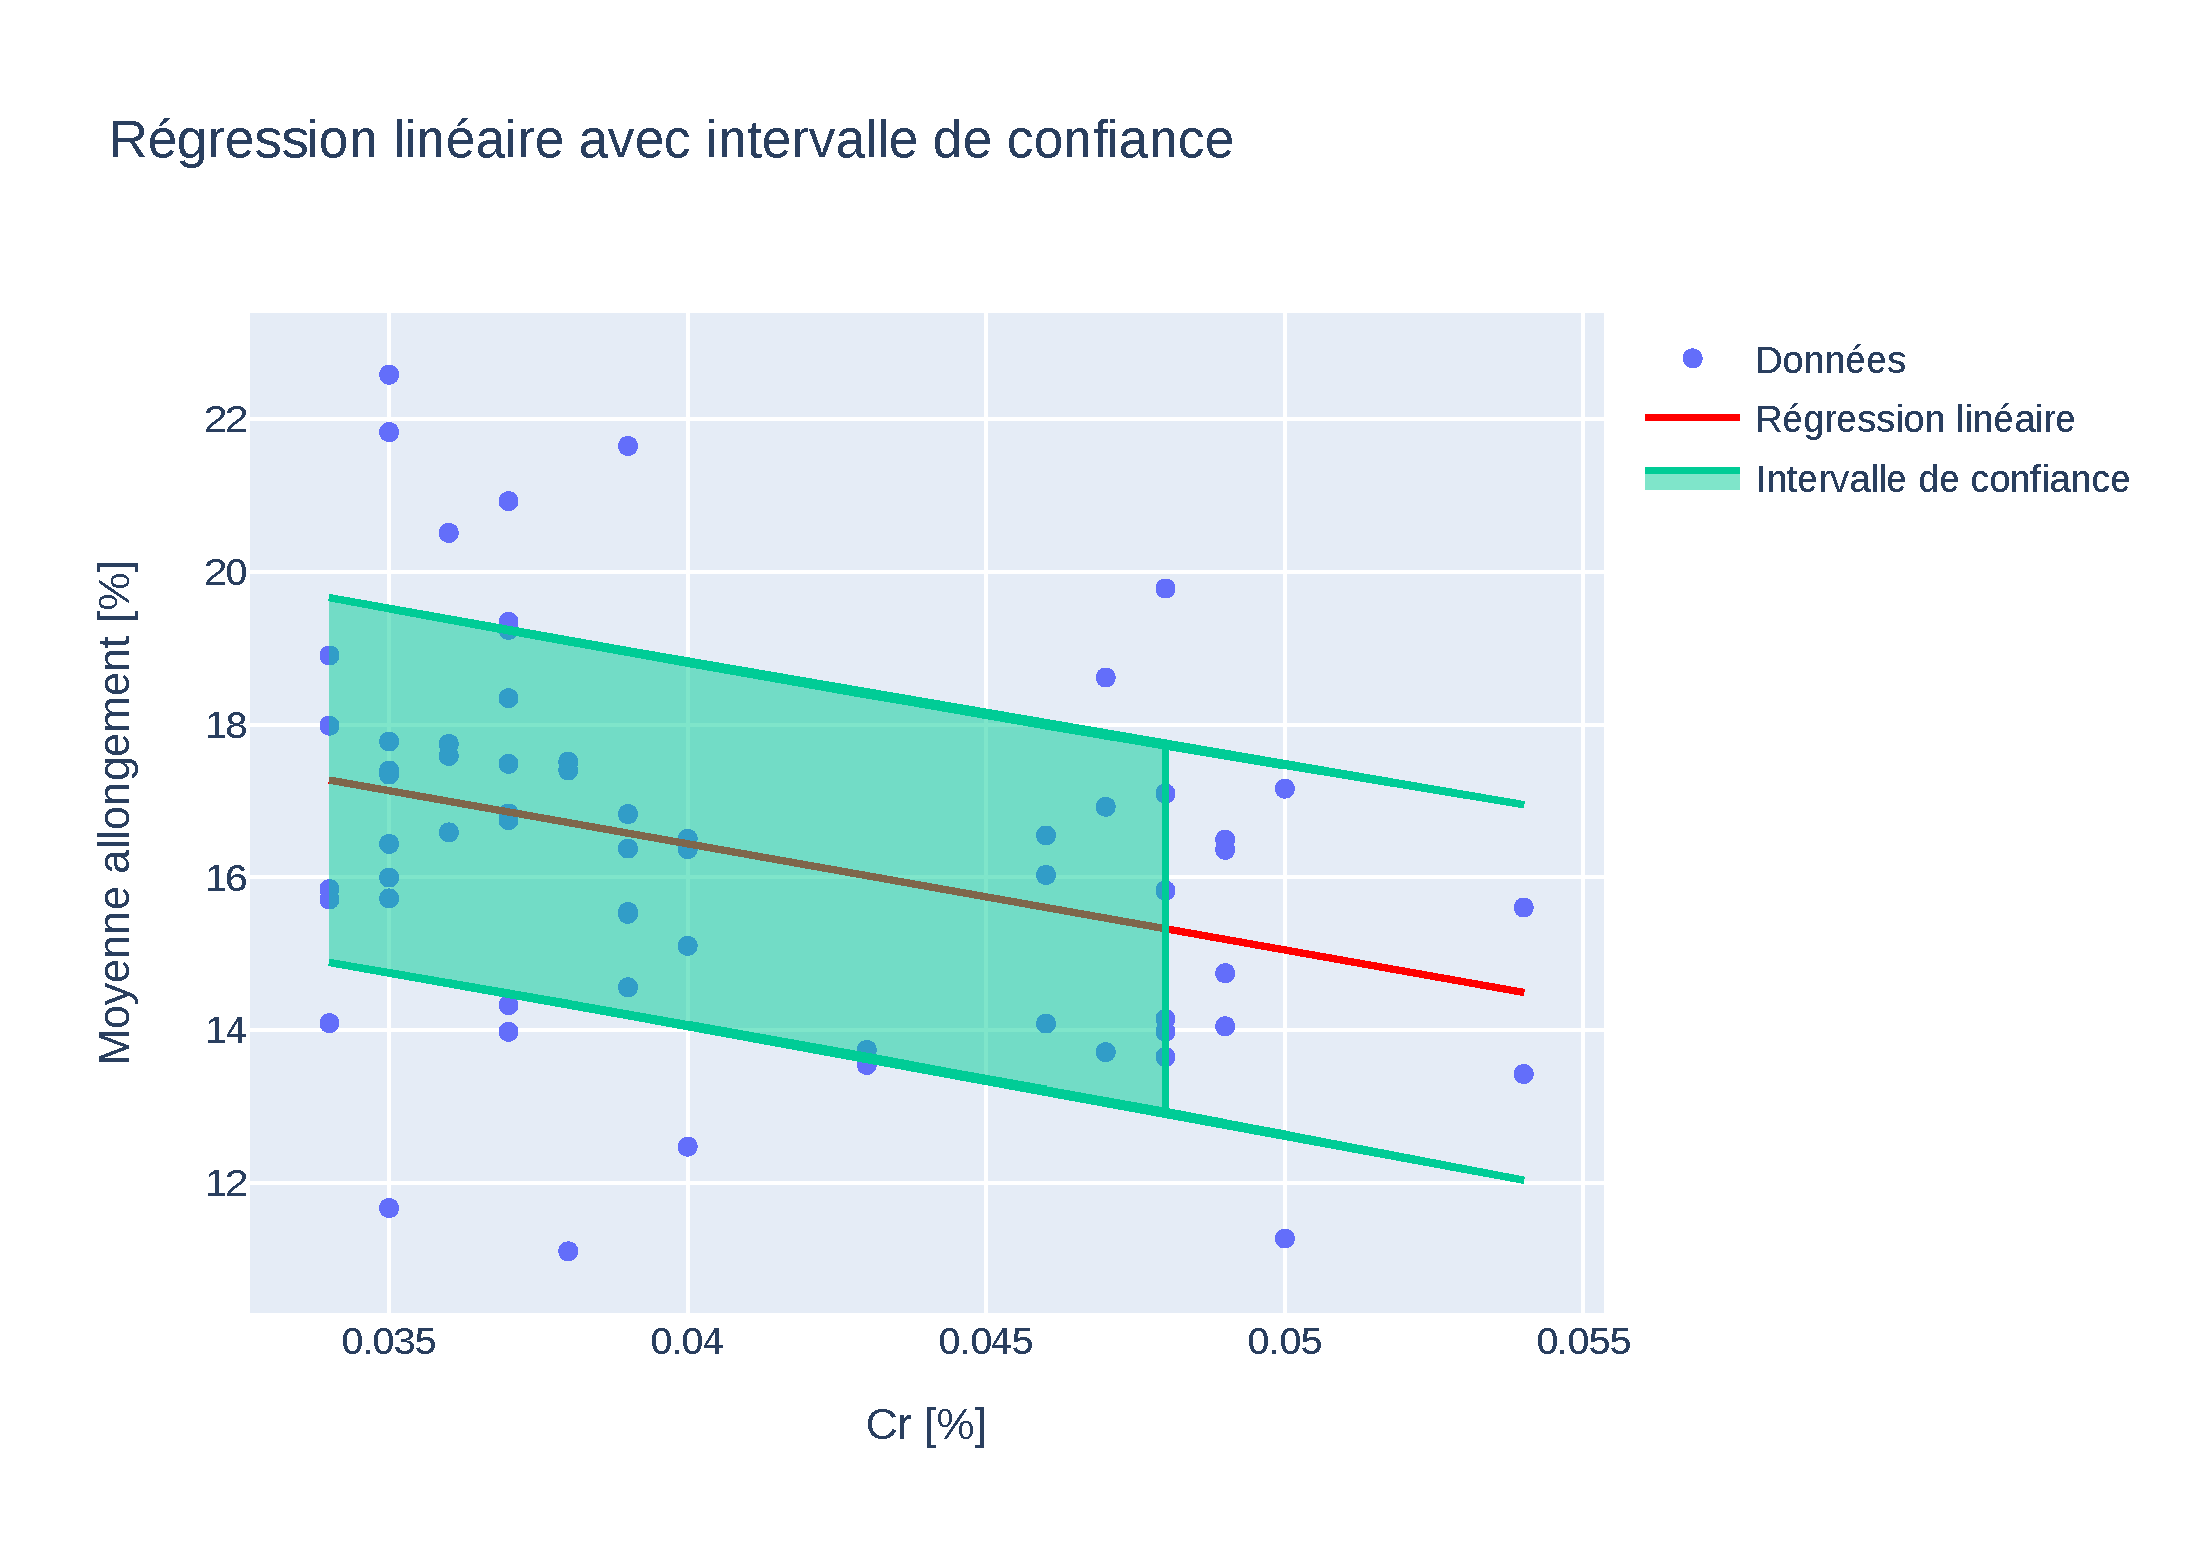
\includegraphics[width=\textwidth]{Figures/Regression_Cr_Allongement.pdf} 
  \end{column}
\end{columns}
\end{frame}


% Allongement
\begin{frame}
\frametitle{Allongement}
\begin{columns}[t]
  \begin{column}{0.5\textwidth}
    \centering
    \textbf{L'allongement en fonction du Cuivre} \\
    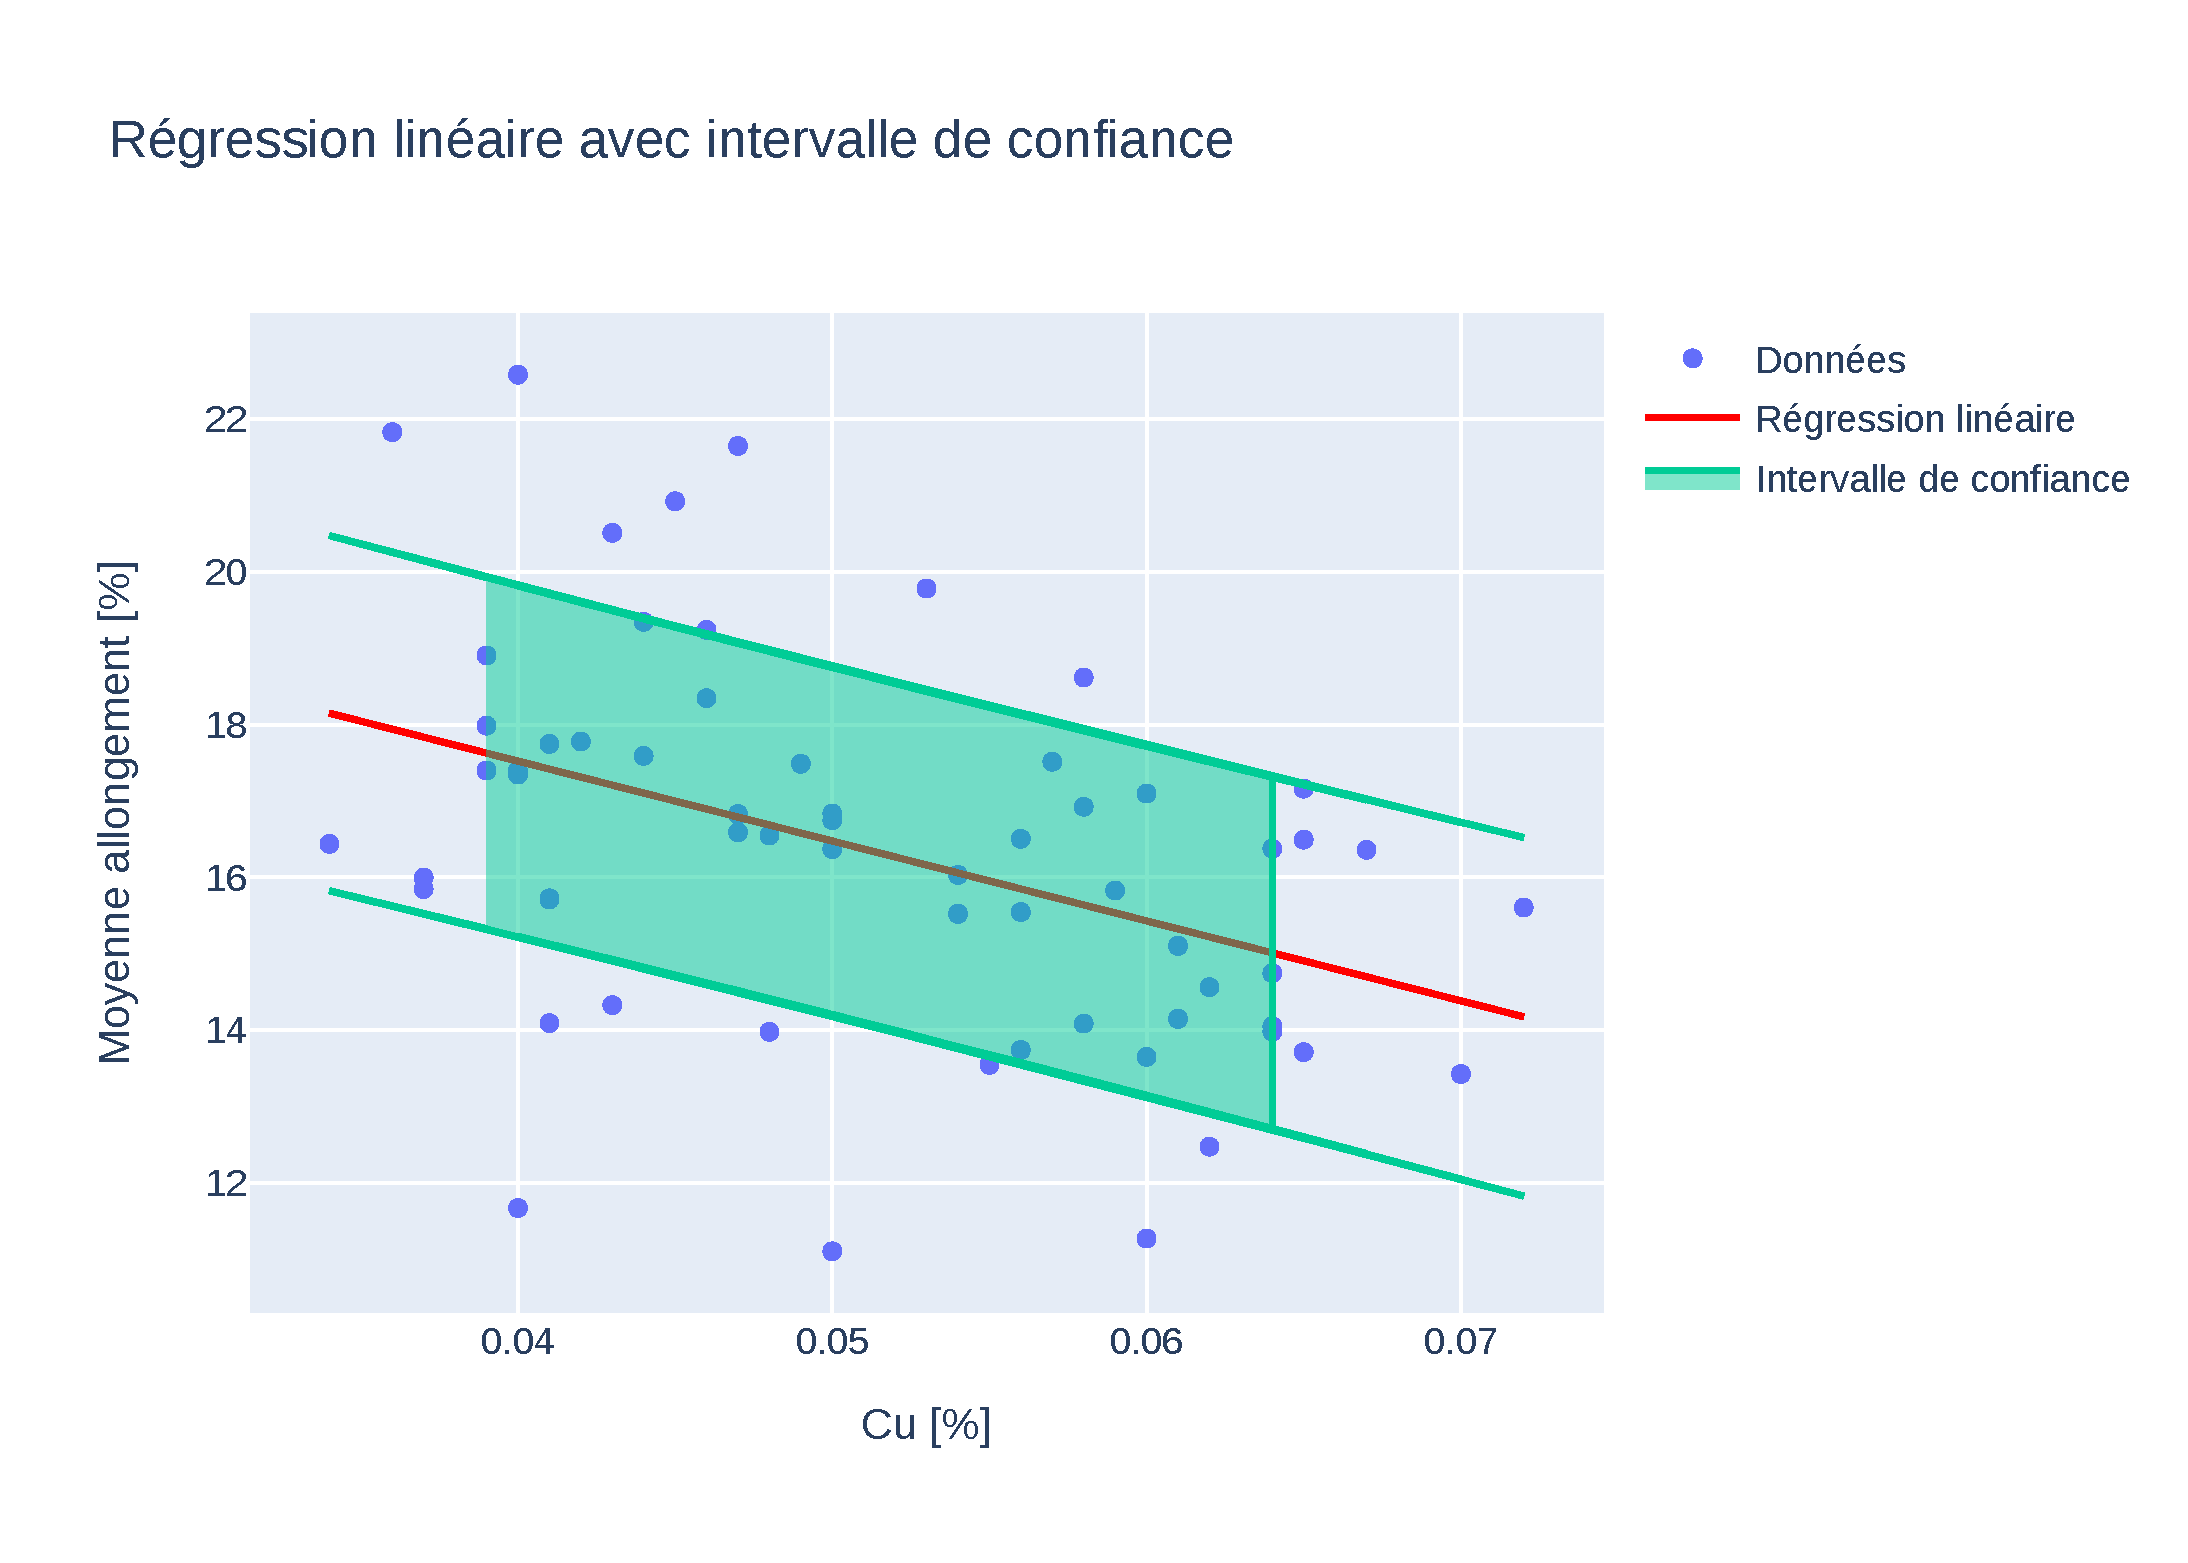
\includegraphics[width=\textwidth]{Figures/Regression_Cu_Allongement.pdf} 
  \end{column}
  \begin{column}{0.5\textwidth}
    \centering
    \textbf{L'allongement en fonction du Sn} \\
    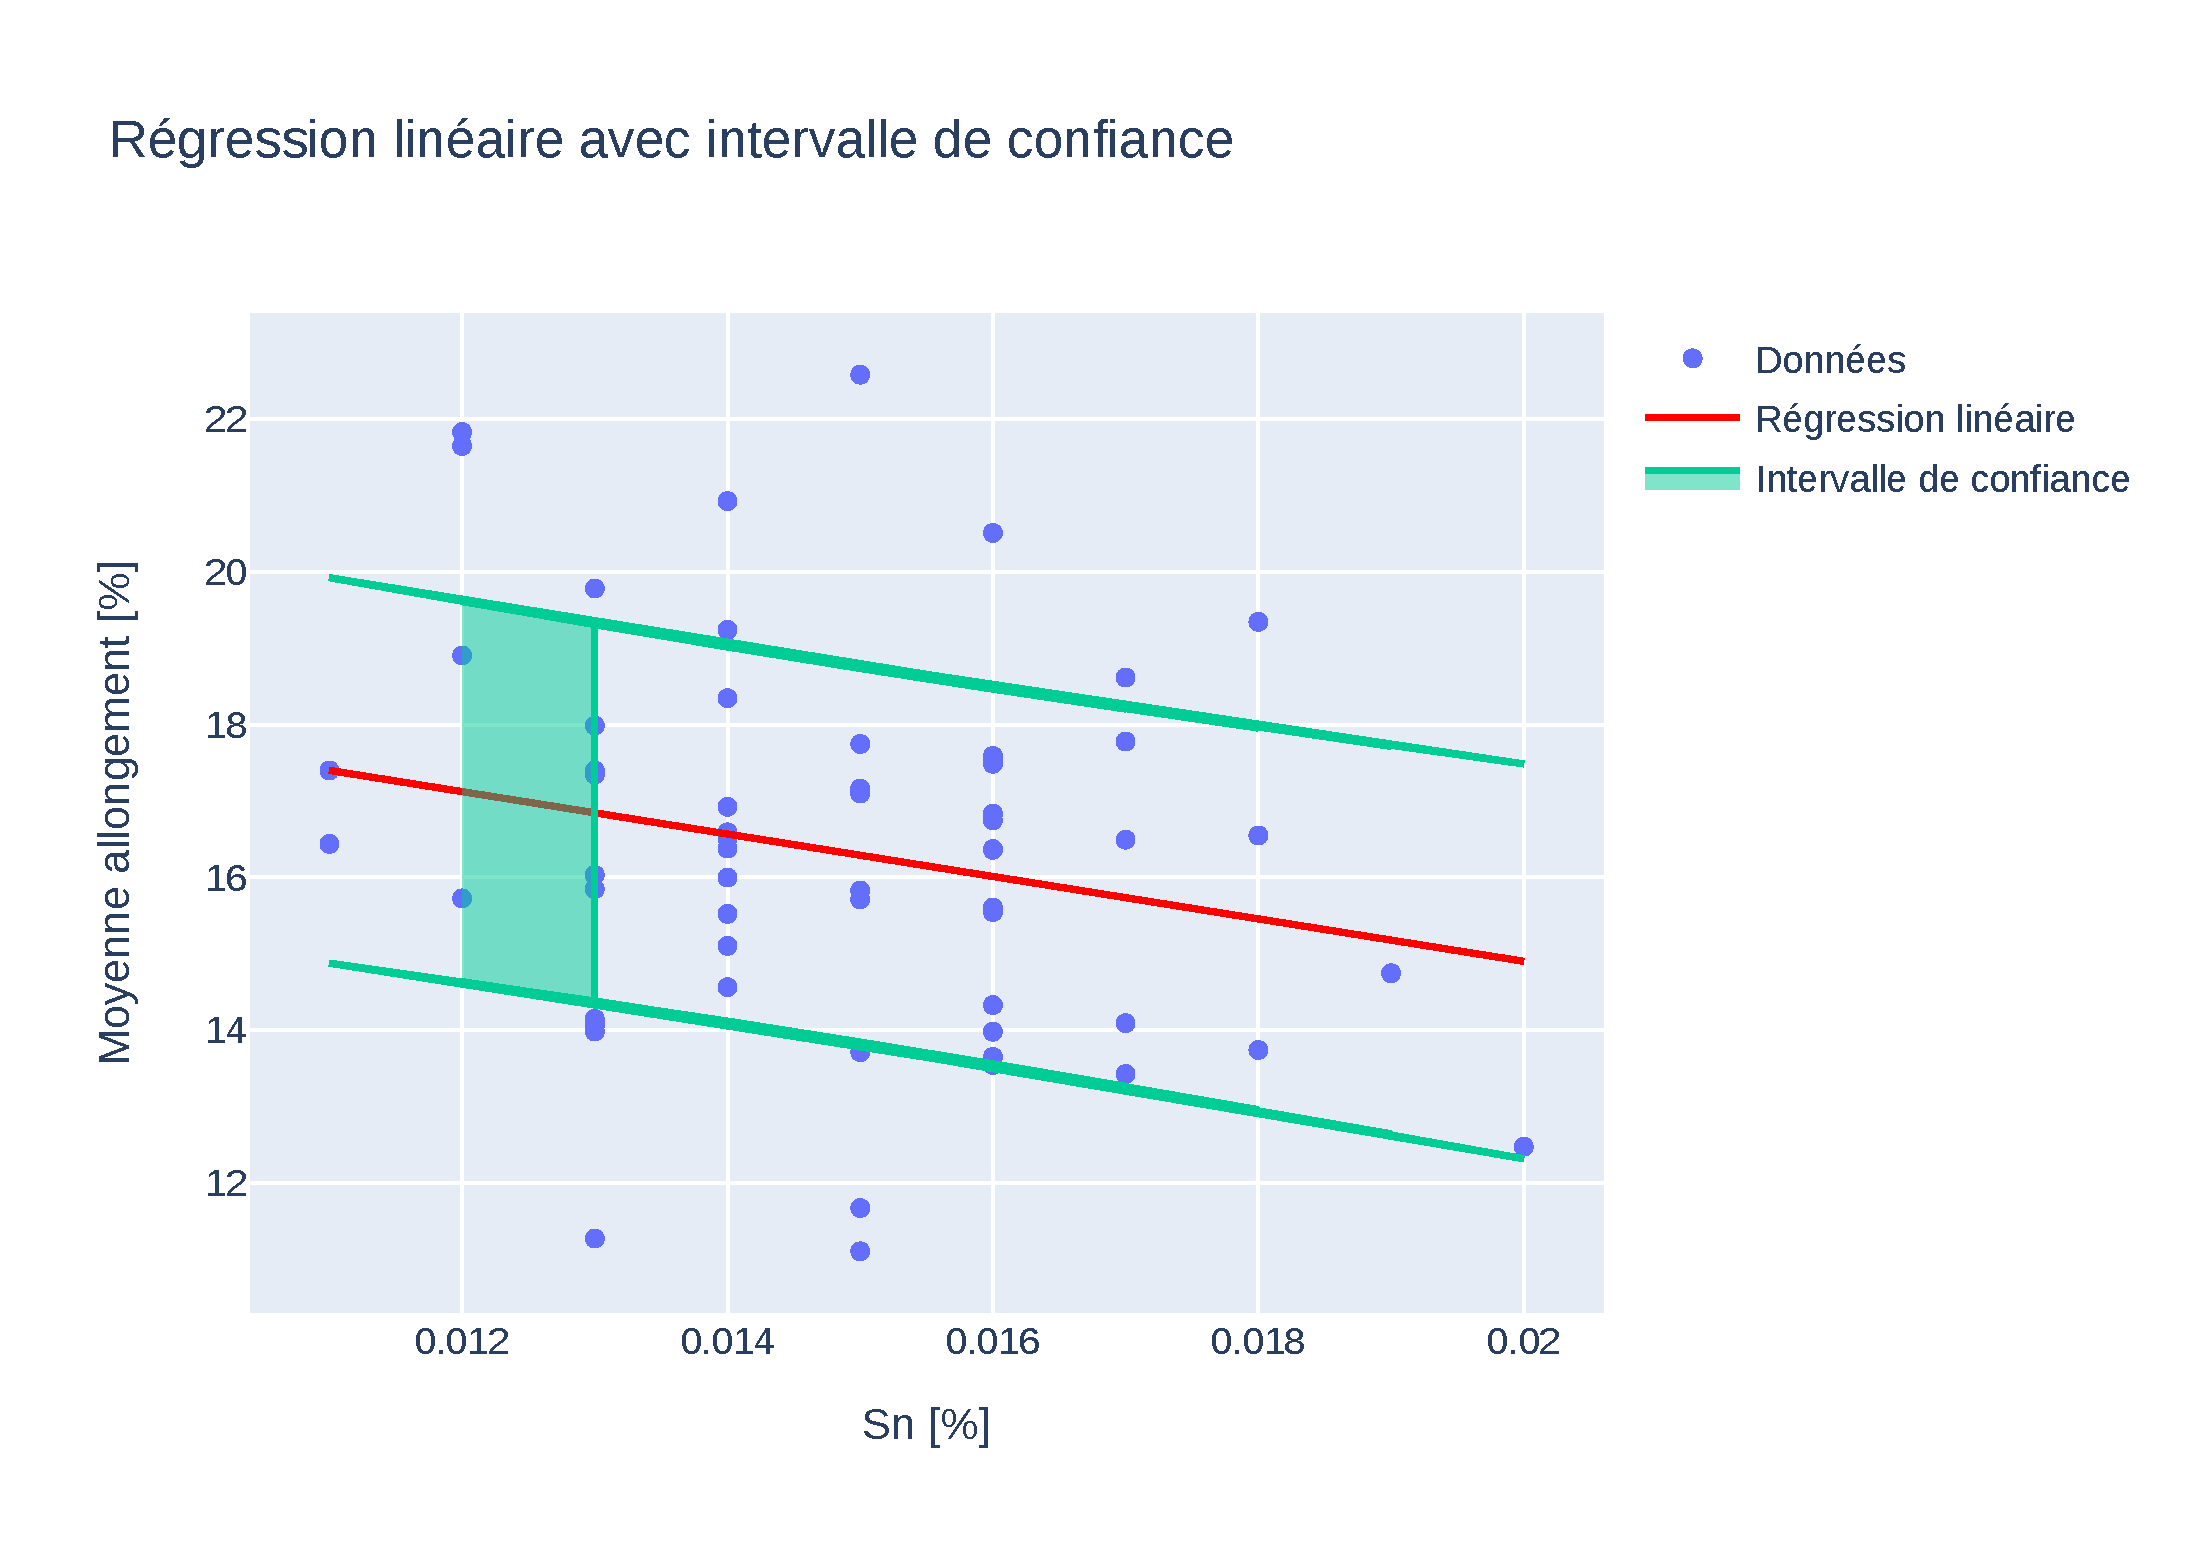
\includegraphics[width=\textwidth]{Figures/Regression_Sn_Allongement.pdf} 
  \end{column}
\end{columns}
\end{frame}




\section{Conclusion}


% Conclusion 
\begin{frame}
\frametitle{Conclusion}
Nous constatons une corrélation linéaire entre le cuivre et la résistance mécanique, ainsi qu'entre le cuivre et l'allongement. En revanche, pour les autres éléments, la linéarité n'est pas  évidente.

\vspace{5pt}

\begin{columns}[t]
\begin{column}{0.5\textwidth}
\textbf{Intervalles de confiance des indicateurs :}
    \begin{itemize}
    \item Impureté : [1.13, 1.19]
    \item Pureté ONO : [0.145, 0.153]
    \end{itemize}
\end{column}
\begin{column}{0.5\textwidth}
\textbf{Intervalles de confiance des éléments chimiques :}
    \begin{itemize}
    \item Sn (Étain) : [0.0143, 0.0153]
    \item Cu (Cuivre) : [0.0488, 0.0538]
    \item Cr (Chrome) : [0.0392, 0.0422]
    \item V (Vanadium) : [0.00092, 0.00111]
    \end{itemize}
\end{column}
\end{columns}
\end{frame}

\begin{frame}
    \begin{center}
        \vfill
        {\Large \bf Thank you for your attention!}\\
    \end{center}
\end{frame}




% \section{References}
% \begin{frame}[allowframebreaks]
%    \bibliography{bibliography}
%     \bibliographystyle{ieeetr}
%    \nocite{*} % used here because no citation happens in slides
%     if there are too many try use:
%     \tiny\bibliographystyle{ieeetr}

% \end{frame}

\end{document}
